\documentclass[12pt,letterpaper]{article}
\usepackage[left=1in,top=1in,right=1in,bottom=1in,nohead]{geometry}
\pagestyle{empty}
\linespread{1.5}
\usepackage[T1]{fontenc}
\usepackage{ragged2e}
\usepackage{setspace}
\usepackage{mdwlist}
% \usepackage{array}
% \usepackage{multirow}
\usepackage{graphicx}
% \usepackage{wrapfig}
% \usepackage{longtable}
% \usepackage{subfig}
\usepackage{amsmath}
\usepackage{amssymb}
\usepackage{bbm}
\usepackage{dsfont}
\usepackage{mathptmx}
\usepackage[hang]{caption}
\DeclareMathAlphabet{\mathcal}{OMS}{cmsy}{m}{n}
\usepackage{relsize}
\usepackage{fancyvrb}
\def \fullline {\vspace{.2em}\hrule\vspace{3px}}

\begin{document}
\tableofcontents
\setlength{\parindent}{0.25in}
\setlength{\floatsep}{0in}
\section{Radial Density Function}
\subsection{Calculation of Distances with Periodicity}
Suppose a large chemical structure has uncountably many atoms but the follow a
periodic pattern of $n$ atoms every $p$ Angstroms. The atom locations within a
period are given by $a_1, a_2, \ldots, a_n$ where $a_i \in \mathbb{R}^3$. The
radial density function is the distribution of pairwise distances between these
atoms.

The distances $d$ between atoms $a_i$ and $a_j$ where $i \neq j$, atom $a_i$
has been displaced by $x$, and atom $a_j$ has been displaced by $y$ per the
periodicity is 
\begin{align*}
  d^2 &= \langle a_i + x - (a_j + y), a_i + x - (a_j + y) \rangle \\
      &= \langle a_i-a_j, a_i-a_j \rangle  + \langle x-y, x-y \rangle  
      + 2 \langle a_i-a_j,x-y \rangle 
\end{align*}
where $x =(k_1 p, k_2 p, k_3 p)$ for $k_i \in \mathbb{Z}$ 
and $y = (l_1 p, l_2 p, l_3 p)$ for $l_i \in \mathbb{Z}$.
Here $\langle x,y \rangle $ denotes the inner product between $x$ and $y$. 

Suppose $D$ is a random variable that samples at random the distances, $d$, in
the chemical structure. The radial density function is the probability density
function of this random variable. This function can be estimated empirically via
a histogram.

The histogram is then normalized by the volume a spherical shell.
\begin{align*}
  \frac{4}{3} &\pi (r + \Delta r)^3 - \frac{4}{3} \pi r^3\\
     &=\frac{4}{3} (3 r^2 \Delta r + 3 r (\Delta r)^2 + (\Delta r)^3) \\
              &\approx 4 \pi r^2 \Delta r
\end{align*}
where $\Delta r$ tends to zero.

For a histogram with frequency, $f$, for bin $[d_i, d_{i+1}]$, we replace $f$
with $f / d_i^2$. And then normalize the histogram so that the sum over all bins
is one.

\subsection{Adding Noise For Atom Vibration}
Due to the vibrations of the molecules, the radial density function will not be
just the equilibrium positions. We can approximate this fluctuation in distances
via a Gaussian filter or Weierstrass transform.

\begin{align*}
F(x)=\frac{1}{\sqrt{4\pi t}} 
  \int_{-\infty}^\infty f(y) e^{-\frac{(x-y)^2}{4t}} dy
\end{align*}

Given that the density function is only defined for a finite number of
distances, we use a discrete version of the transform making sure to keep the
sum of the weights equal to one.

\begin{align*}
  F(d_k) = \frac{\sum_{d_i = d_0}^{d_n} f(d_i) \exp\left(-\frac{(d_k -
                  d_i)^2}{4t}\right)}
            {\sum_{d_i = d_0}^{d_n} \exp\left(-\frac{(d_k - d_i)^2}{4t}\right)}
\end{align*}
where $d_0$ is the minimum distance and $d_n$ is the maximum distance.

\subsection{Cubane Example}
As an example of the above, below are the calculations for cubane ($C_8 H_8$).\\

\noindent Here are the coordinates of the elements in cubane in Angstroms.

\begin{verbatim}
Element, x, y, z
C, 1.2455, 0.5367,-0.0729
C, 0.9239,-0.9952, 0.0237
C,-0.1226,-0.7041, 1.1548
C, 0.1989, 0.8277, 1.0582
C, 0.1226, 0.7042,-1.1548
C,-0.9239, 0.9952,-0.0237
C,-1.2454,-0.5367, 0.0729
C,-0.1989,-0.8277,-1.0582
H, 2.2431, 0.9666,-0.1313
H, 1.6638,-1.7924, 0.0426
H,-0.2209,-1.2683, 2.0797
H, 0.3583, 1.4907, 1.9059
H, 0.2208, 1.2681,-2.0799
H,-1.6640, 1.7922,-0.0427
H,-2.2430,-0.9665, 0.1313
H,-0.3583,-1.4906,-1.9058
\end{verbatim}

\subsubsection{Cubane Radial Density Functions}
\begin{figure}[ht!]
  \begin{center}
    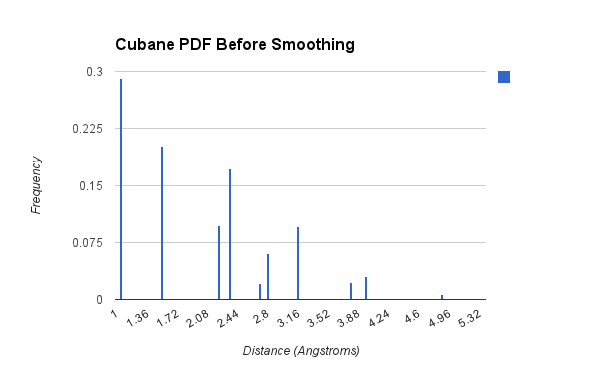
\includegraphics[scale=0.7]{figs/cubane_rdf_before_smoothing.png}
    \caption{Before Smoothing}
  \end{center}
\end{figure}

\begin{figure}[ht!]
  \begin{center}
    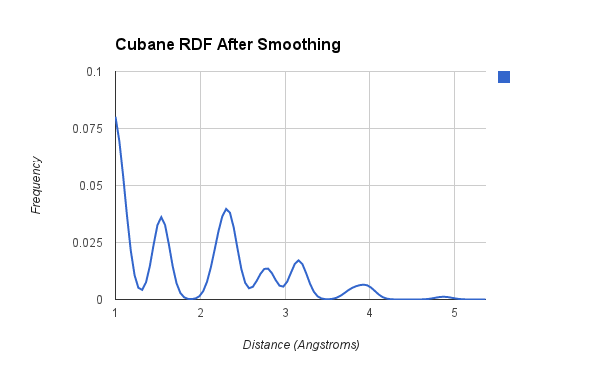
\includegraphics[scale=0.7]{figs/cubane_rdf_after_smoothing.png}
    \caption{After Smoothing}
  \end{center}
\end{figure}
\clearpage

\subsection{Experimental and Theoretical RDFs for Known Structures}
For some structures, we are able to theoretically calculate the RDF from atom
locations and also have the experimental RDF from Xray scattering. These known
matches provide some insight into understanding how the experiments and theory
align. The RDF comparison are shown below.

Outside of these structures, there are not many other known matches. There are a
few reasons for this. First, if a structures is already known at the atomic
level then there is no need to run an xray diffraction experiment. Second, if a
structure is periodic as in a lattice, the atomic structure can be determined by
xray diffraction which is easier and cheaper than xray scattering.

\subsubsection{Ga As}
\noindent Experimental Data: Pair Distribution Functions Analysis, Valeri
Petkov\\
\noindent Calculated Data: Maria Chan\\
\begin{figure}[ht]
  \begin{center}
    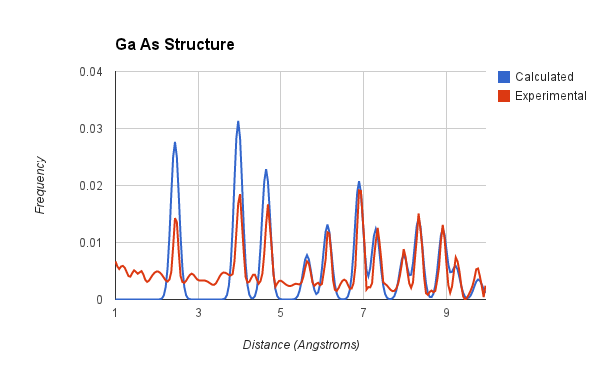
\includegraphics[scale=0.7]{figs/gaas_rdf_comparison.png}
    \caption{Ga As}
  \end{center}
\end{figure}

\subsubsection{In As}
\noindent Experimental Data: Pair Distribution Functions Analysis, Valeri
Petkov\\
\noindent Calculated Data: Maria Chan\\
\begin{figure}[ht]
  \begin{center}
    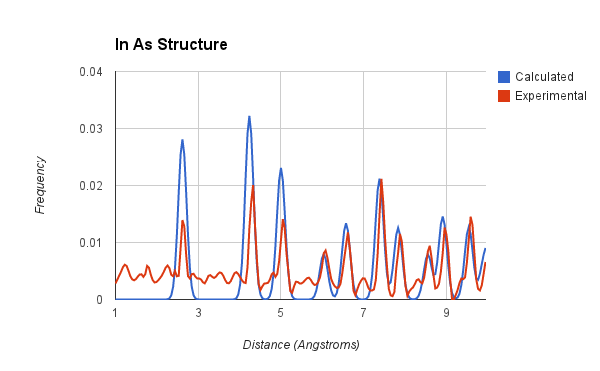
\includegraphics[scale=0.7]{figs/inas_rdf_comparison.png}
    \caption{In As}
  \end{center}
\end{figure}

\subsubsection{Si Lattice}
\noindent Experimental Data: J. AM. CHEM. SOC. VOL. 133, NO. 3, 2011, P:
503-512\\
\noindent Calculated Data: http://materialsproject.org/materials/mp-149/ \\
\begin{figure}[ht]
  \begin{center}
    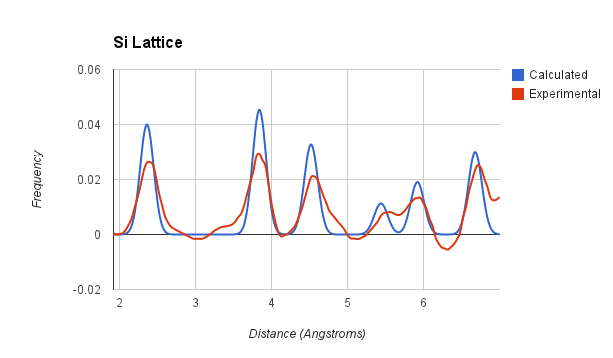
\includegraphics[scale=0.7]{figs/si_lattice_comparison.png}
    \caption{Si Lattice}
  \end{center}
\end{figure}

\pagebreak

\section{Noise Analysis}
% exp noise example
% peak counts: estimation method, histogram, dist
% peak location: estimation method, histogram, dist
% noise peak heights: estimation method, histogram, dist
% example noisy images
% peak counts for max lengths
\subsection{Peak Counts}
\begin{figure}[ht]
  \begin{center}
    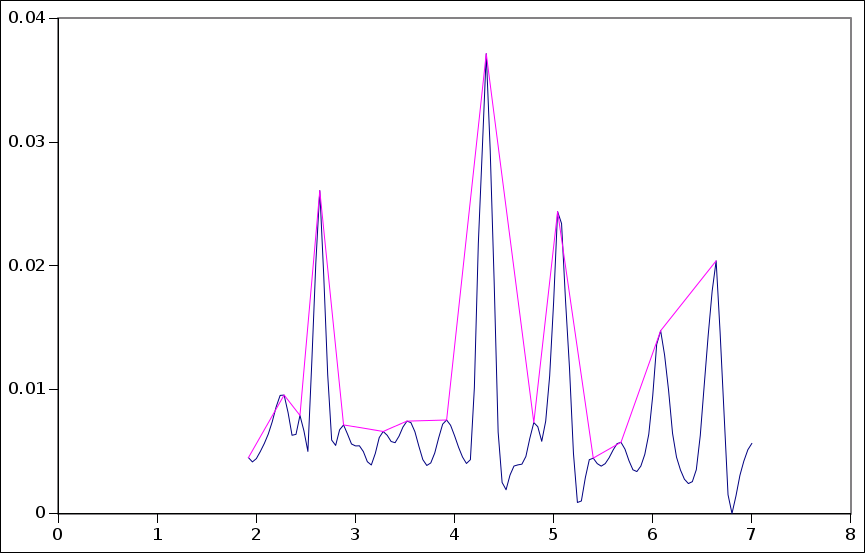
\includegraphics[scale=0.5]{figs/inas_peaks_7ang.png}
    \caption{InAs Expt, Max 7 Angstroms}
  \end{center}
\end{figure}

\begin{figure}[ht]
  \begin{center}
    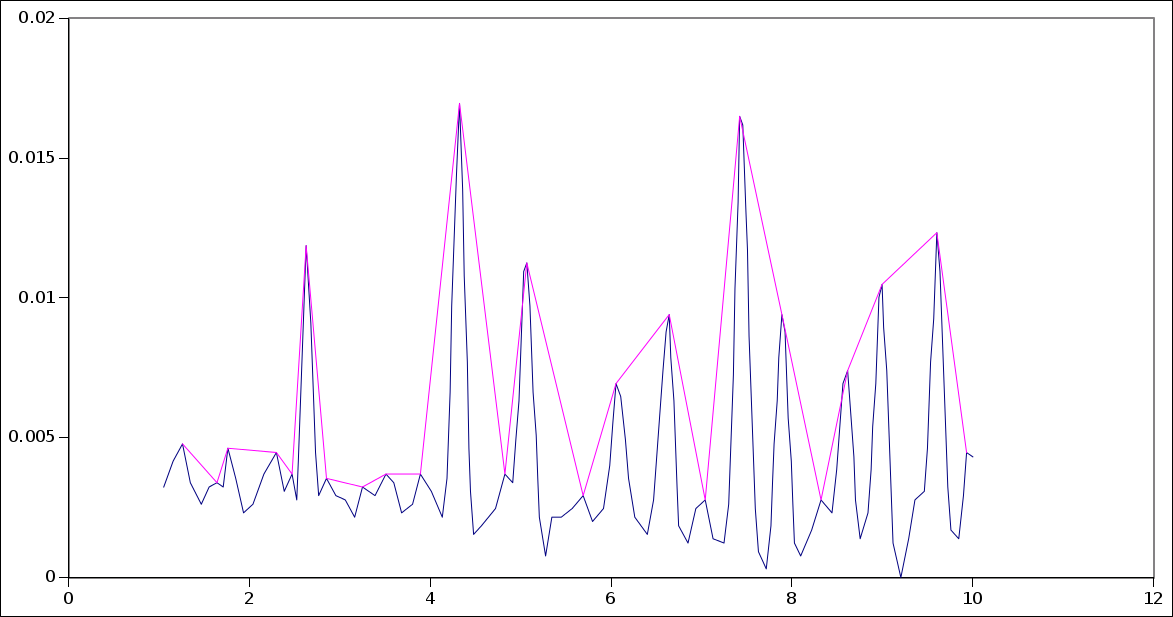
\includegraphics[scale=0.4]{figs/inas_peaks_10ang.png}
    \caption{InAs Expt, Max 10 Angstroms}
  \end{center}
\end{figure}
\clearpage

\section{Recognition Using Eigenfaces}
% experimental accuracy - by pca dim
% synthetic accuracy - by pca dim
\subsection{Mean Image}
\begin{figure}[ht]
  \begin{center}
    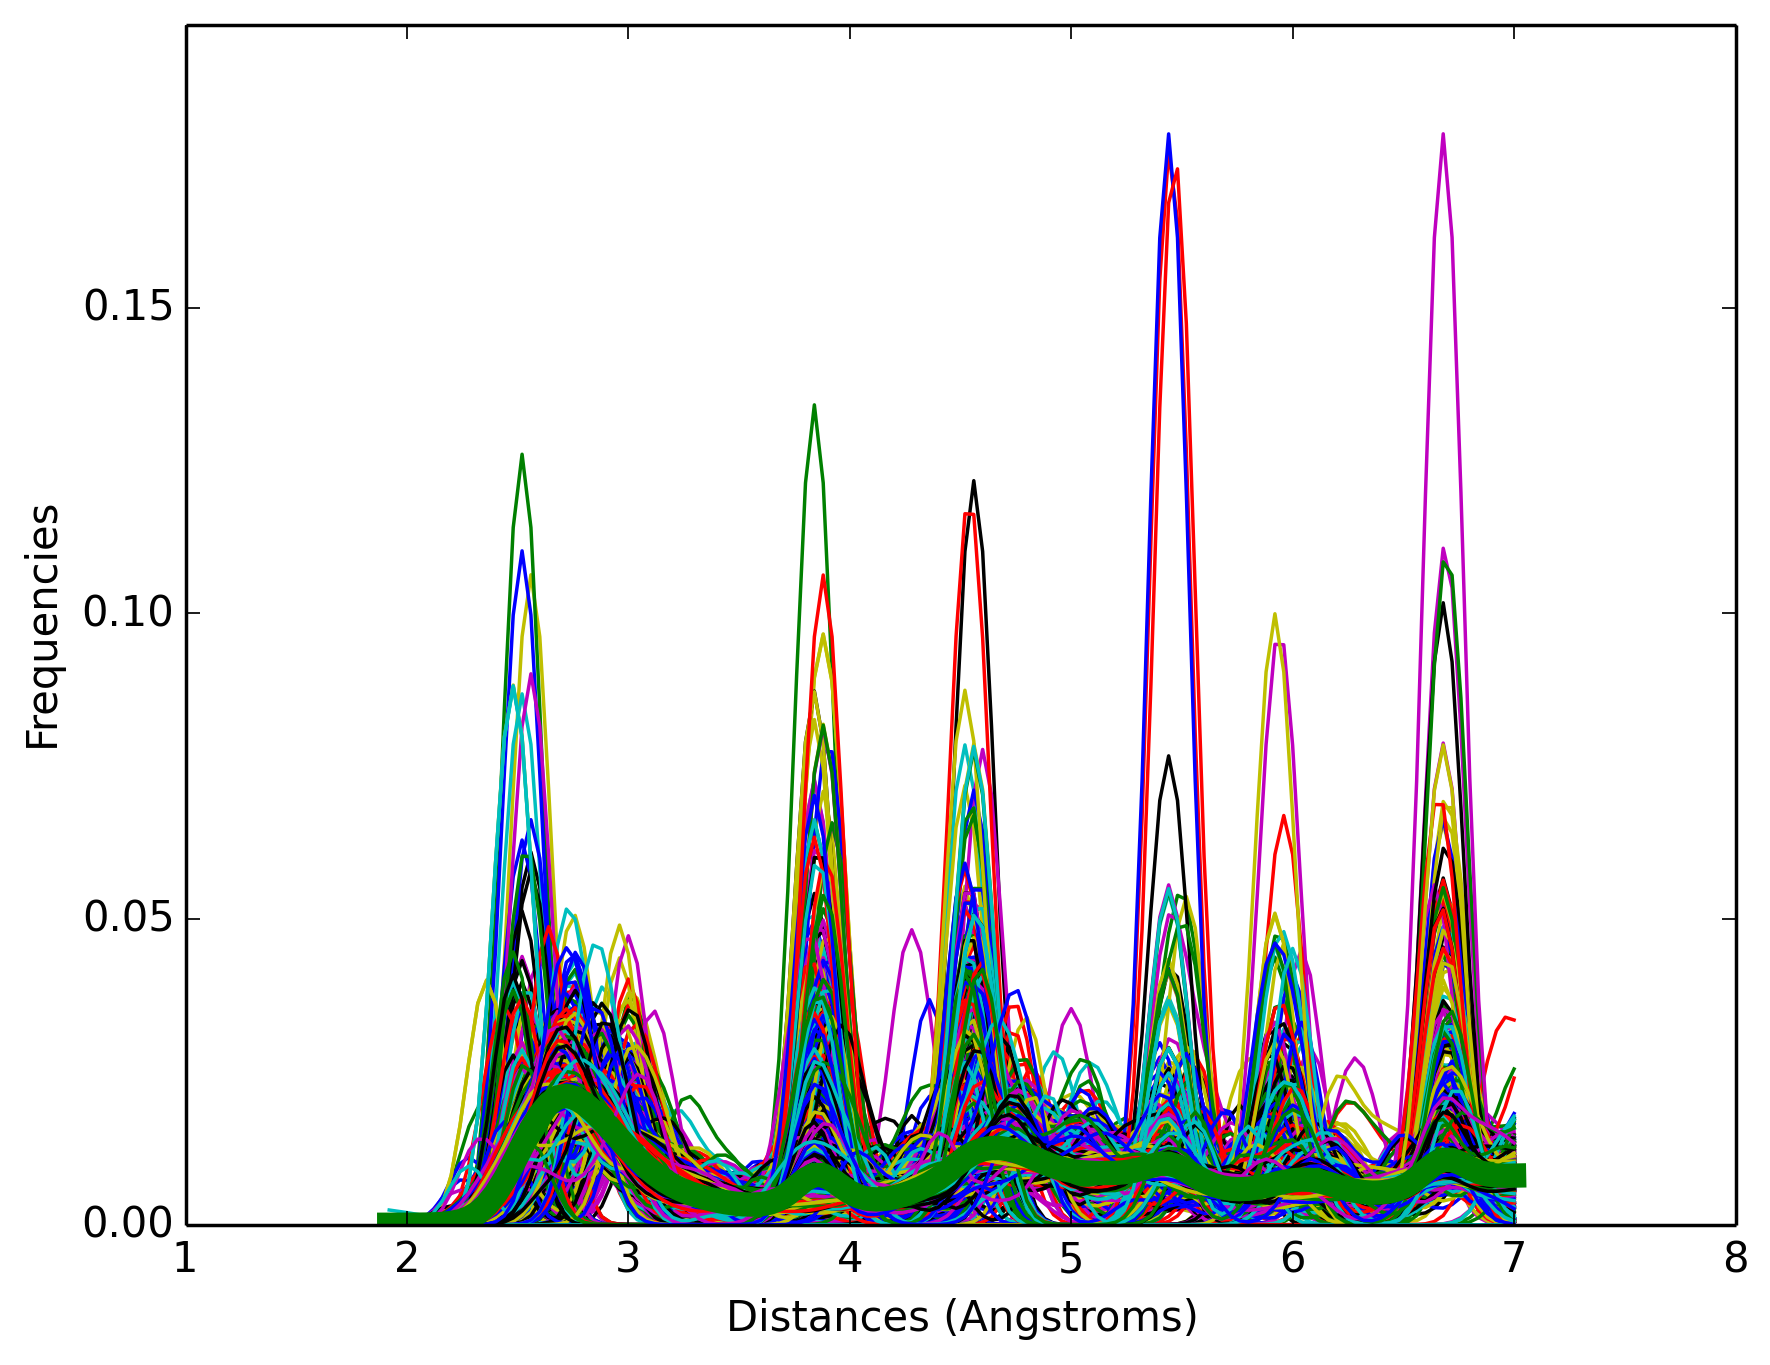
\includegraphics[scale=0.8]{figs/all_calc_images_mean.png}
    \caption{All Calculated Images with Mean}
  \end{center}
\end{figure}
\clearpage

\subsection{Variance Explained by Principal Components}
\begin{figure}[ht]
  \begin{center}
    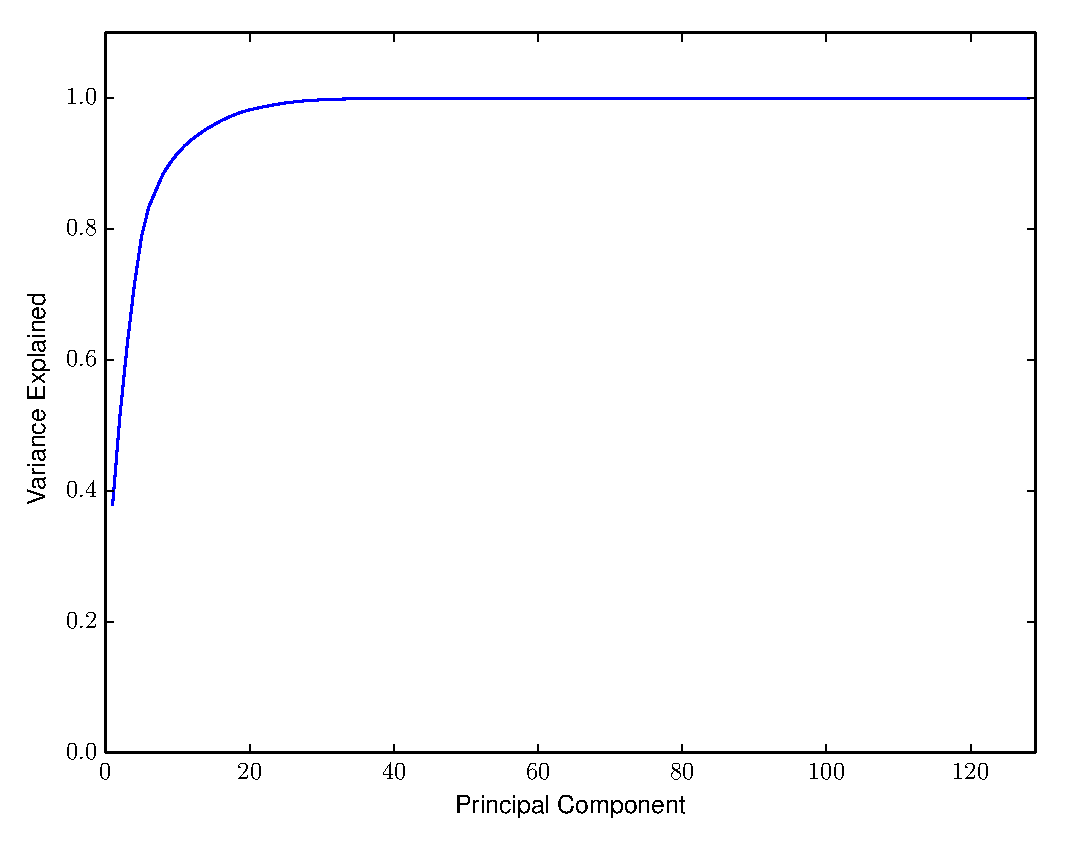
\includegraphics[scale=0.8]{figs/eigenfaces_varexplained.eps}
    \caption{Cumulative Variance Explained by Principal Components}
  \end{center}
\end{figure}
\clearpage

\subsection{Eigenfaces}
\begin{figure}[ht]
  \begin{center}
    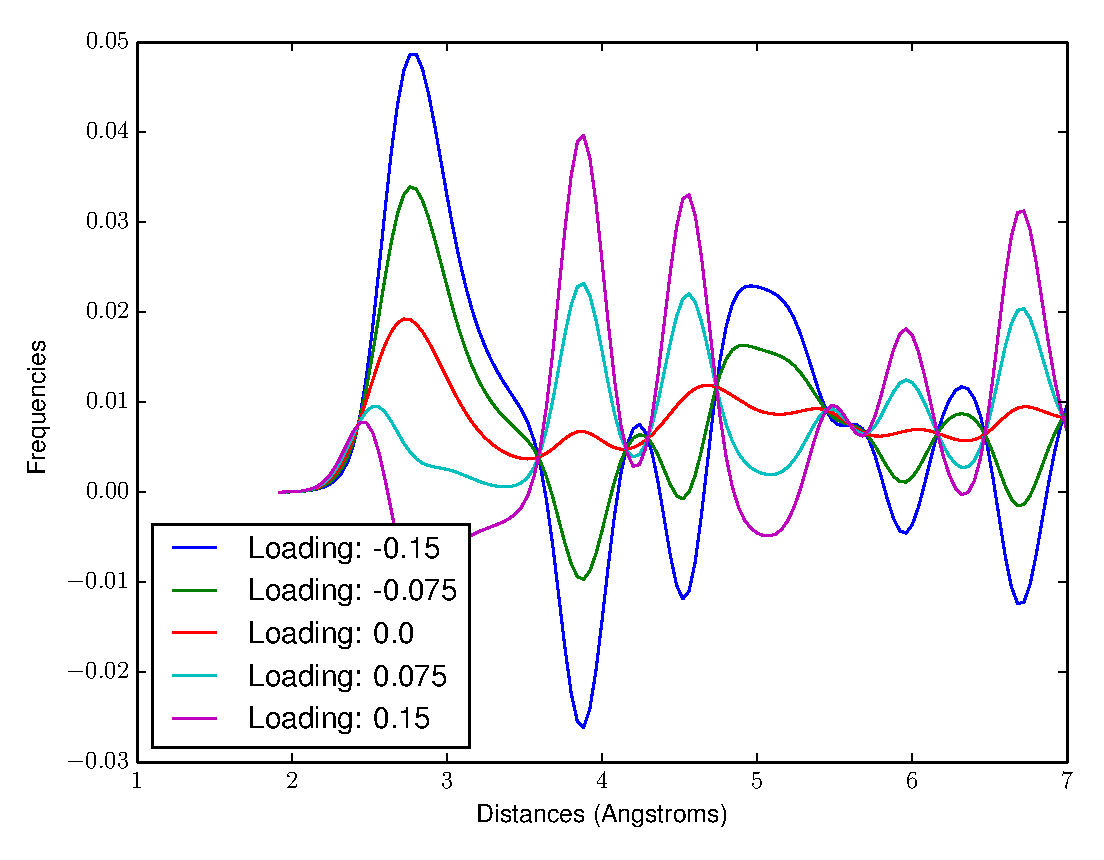
\includegraphics[scale=0.8]{figs/eigenface1.eps}
    \caption{First Eigenface}
  \end{center}
\end{figure}

\begin{figure}[ht]
  \begin{center}
    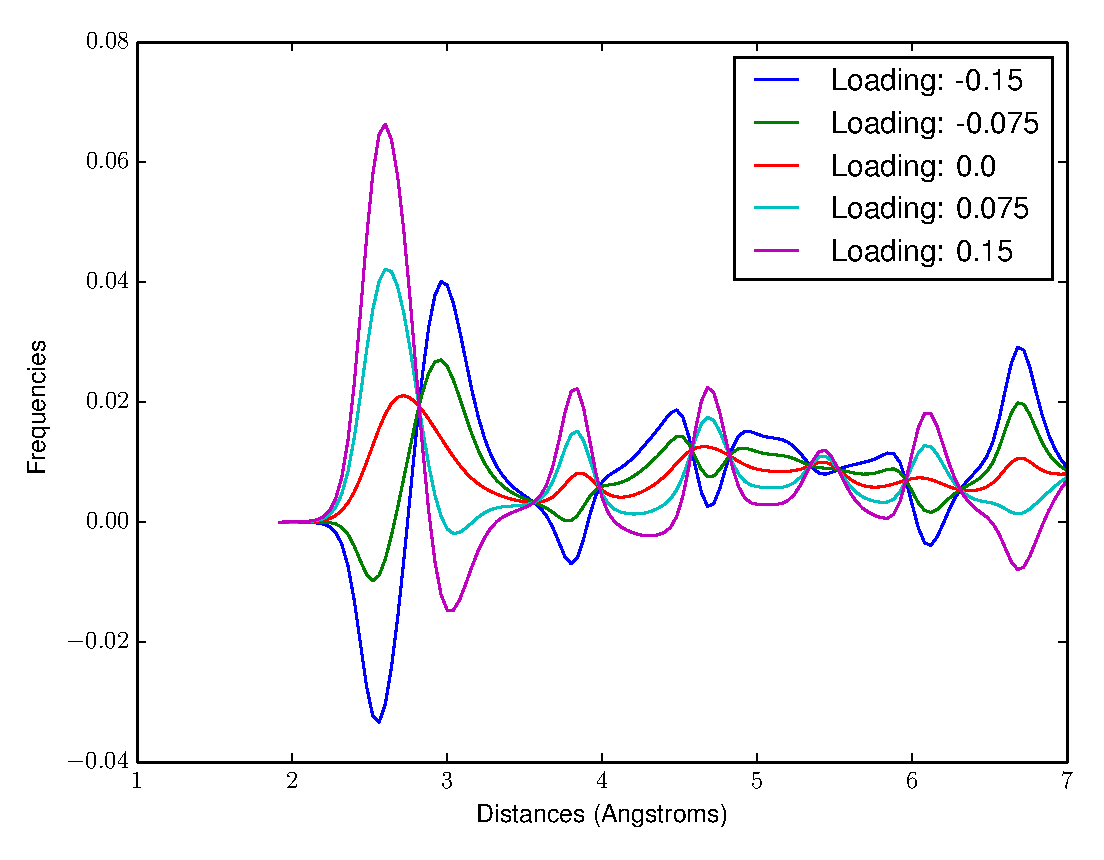
\includegraphics[scale=0.8]{figs/eigenface2.eps}
    \caption{Second Eigenface}
  \end{center}
\end{figure}

\begin{figure}[ht]
  \begin{center}
    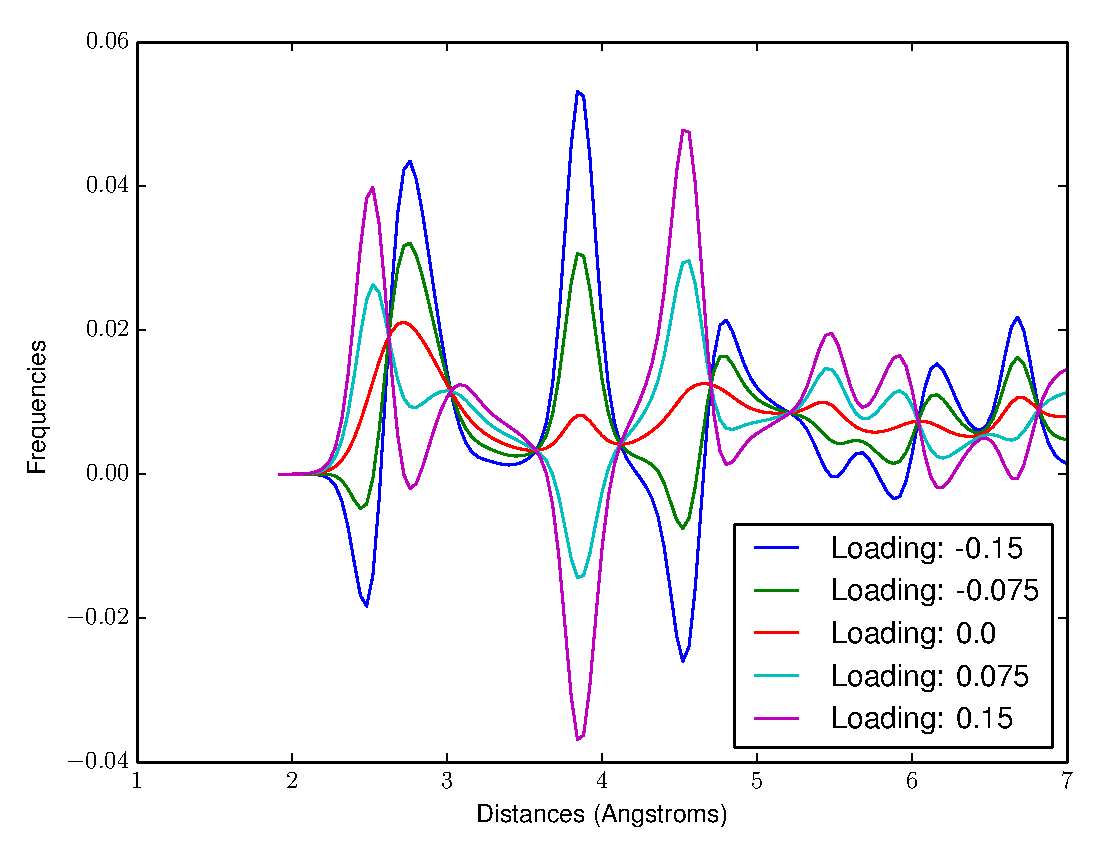
\includegraphics[scale=0.8]{figs/eigenface3.eps}
    \caption{Third Eigenface}
  \end{center}
\end{figure}
\clearpage

\subsection{Data in Eigenspace}
\begin{figure}[ht]
  \begin{center}
    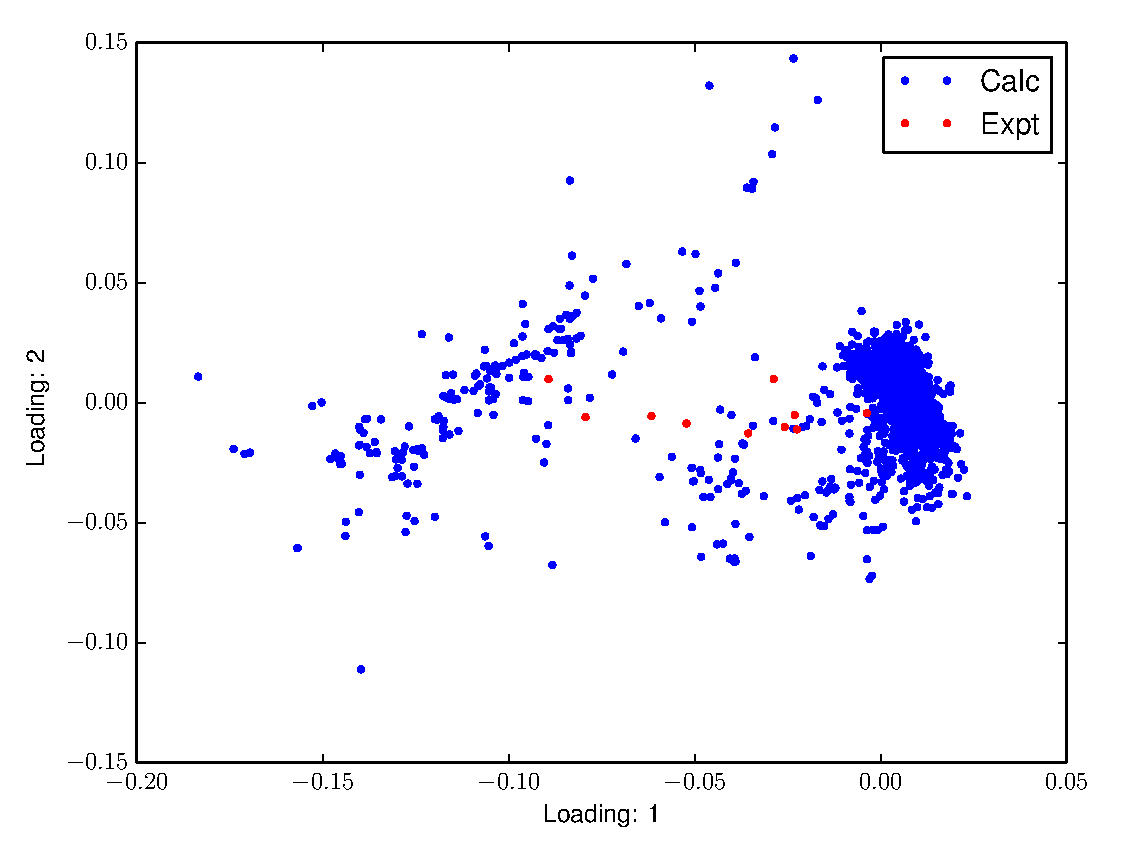
\includegraphics[scale=0.8]{figs/eigenspace1-2.eps}
    \caption{Loading 1 vs  Loading 2}
  \end{center}
\end{figure}

\begin{table}[ht]
  \begin{center}
  \begin{tabular}{|l|l|l|}
    \hline
    \textbf{Label} & \textbf{Loading 1} & \textbf{Loading 2} \\ \hline
    SiLiExpt1      & -0.0893            & 0.00982            \\ \hline
    SiLiExpt2      & -0.0794            & -0.006             \\ \hline
    SiLiExpt3      & -0.0616            & -0.0055            \\ \hline
    SiLiExpt4      & -0.0522            & -0.0086            \\ \hline
    SiLiExpt5      & -0.0356            & -0.0128            \\ \hline
    ExptGaAs       & -0.0288            & 0.00994            \\ \hline
    SiLiExpt7      & -0.0258            & -0.0101            \\ \hline
    SiLiExpt6      & -0.0231            & -0.0051            \\ \hline
    SiLiExpt8      & -0.0226            & -0.0111            \\ \hline
    ExptInAs       & -0.0038            & -0.0044            \\ \hline
  \end{tabular}
  \caption{Experimental Data Sorted by Loading 1}
  \end{center}
\end{table}

\begin{table}[h]
  \begin{center}
  \begin{tabular}{|l|l|l|}
    \hline
    \textbf{Label} & \textbf{Loading 1} & \textbf{Loading 2} \\ \hline
    SiLiExpt5      & -0.0356            & -0.0128            \\ \hline
    SiLiExpt8      & -0.0226            & -0.0111            \\ \hline
    SiLiExpt7      & -0.0258            & -0.0101            \\ \hline
    SiLiExpt4      & -0.0522            & -0.0086            \\ \hline
    SiLiExpt2      & -0.0794            & -0.006             \\ \hline
    SiLiExpt3      & -0.0616            & -0.0055            \\ \hline
    SiLiExpt6      & -0.0231            & -0.0051            \\ \hline
    ExptInAs       & -0.0038            & -0.0044            \\ \hline
    SiLiExpt1      & -0.0893            & 0.00982            \\ \hline
    ExptGaAs       & -0.0288            & 0.00994            \\ \hline
  \end{tabular}
  \caption{Experimental Data Sorted by Loading 2}
  \end{center}
\end{table}

\begin{figure}[ht]
  \begin{center}
    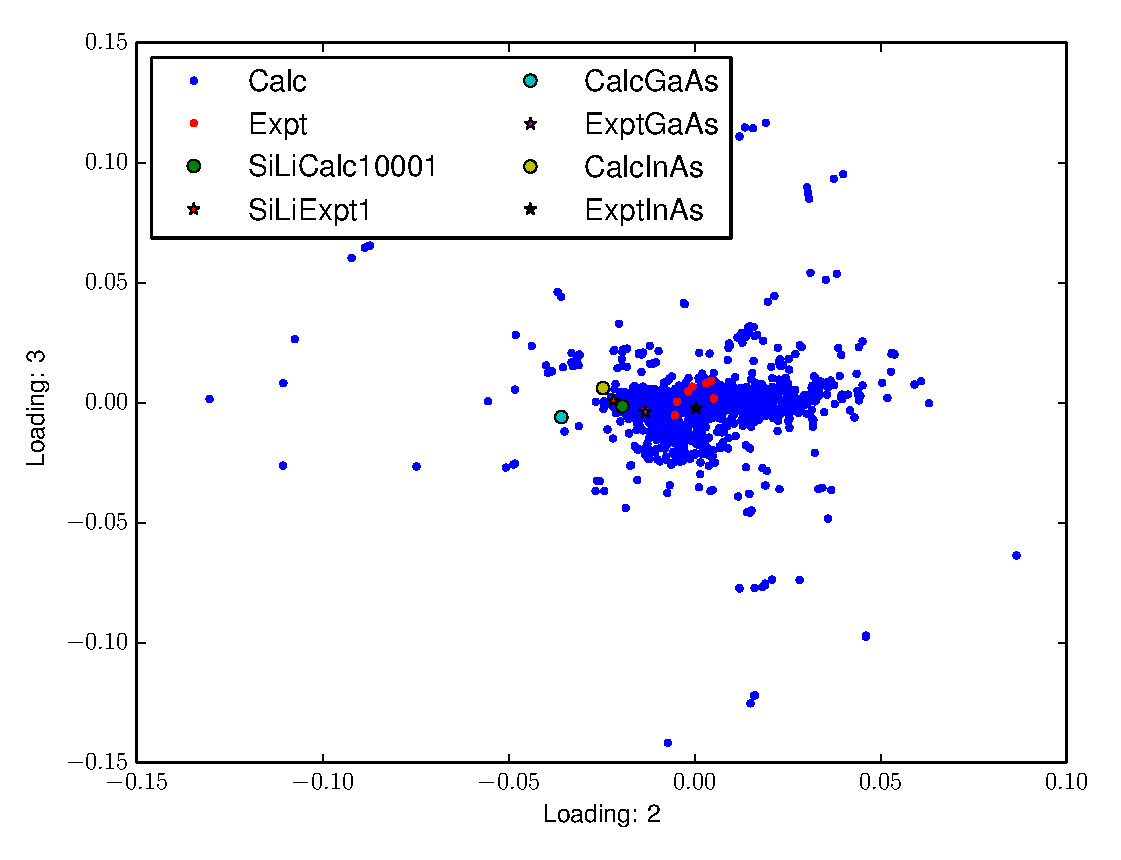
\includegraphics[scale=0.8]{figs/eigenspace2-3.eps}
    \caption{Loading 2 vs  Loading 3}
  \end{center}
\end{figure}

\begin{figure}[ht]
  \begin{center}
    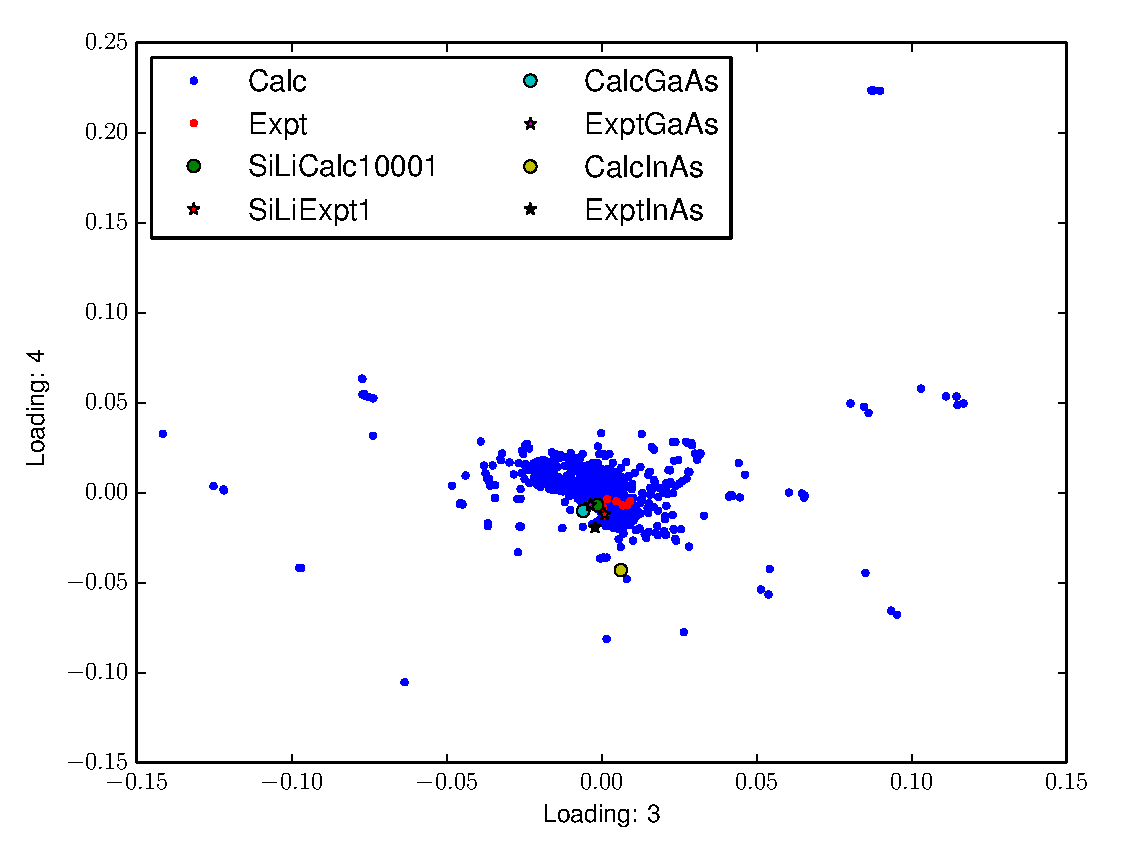
\includegraphics[scale=0.8]{figs/eigenspace3-4.eps}
    \caption{Loading 3 vs  Loading 4}
  \end{center}
\end{figure}

\begin{figure}[ht]
  \begin{center}
    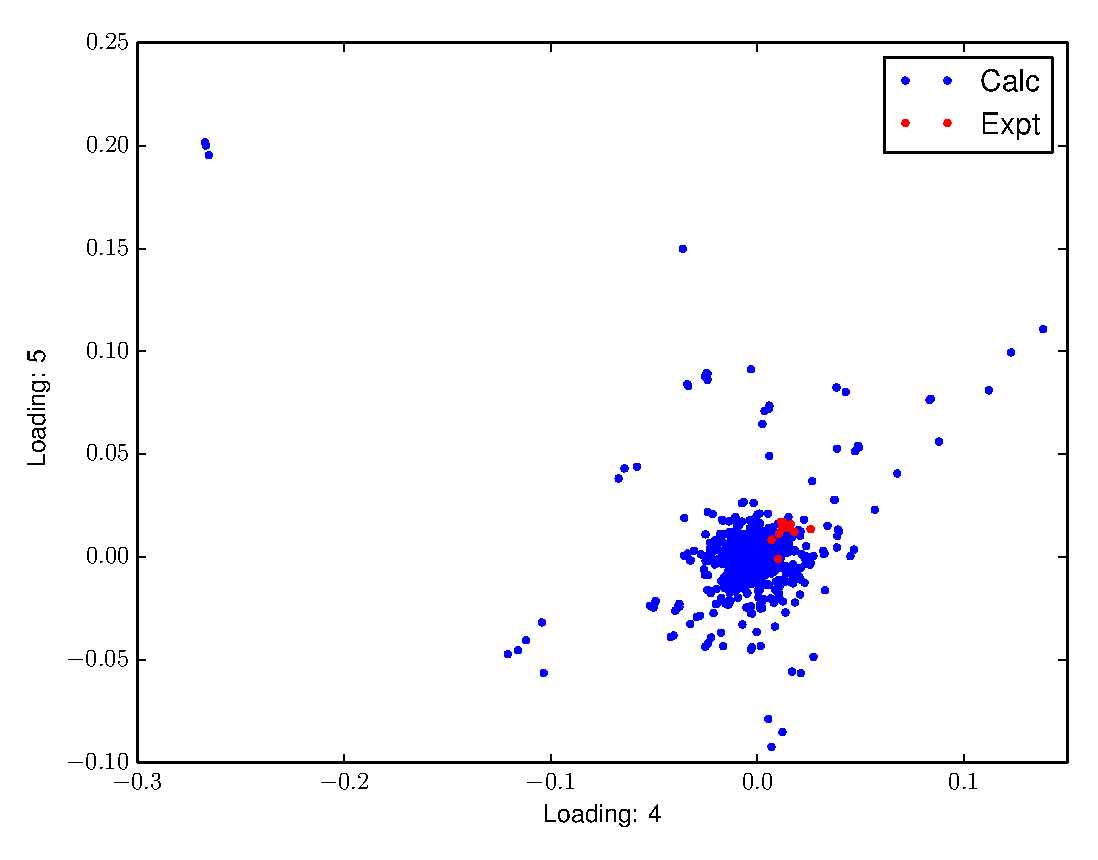
\includegraphics[scale=0.8]{figs/eigenspace4-5.eps}
    \caption{Loading 4 vs  Loading 5}
  \end{center}
\end{figure}
\clearpage

\subsubsection{Eigenspace Outliers}
\begin{figure}[ht]
  \begin{center}
    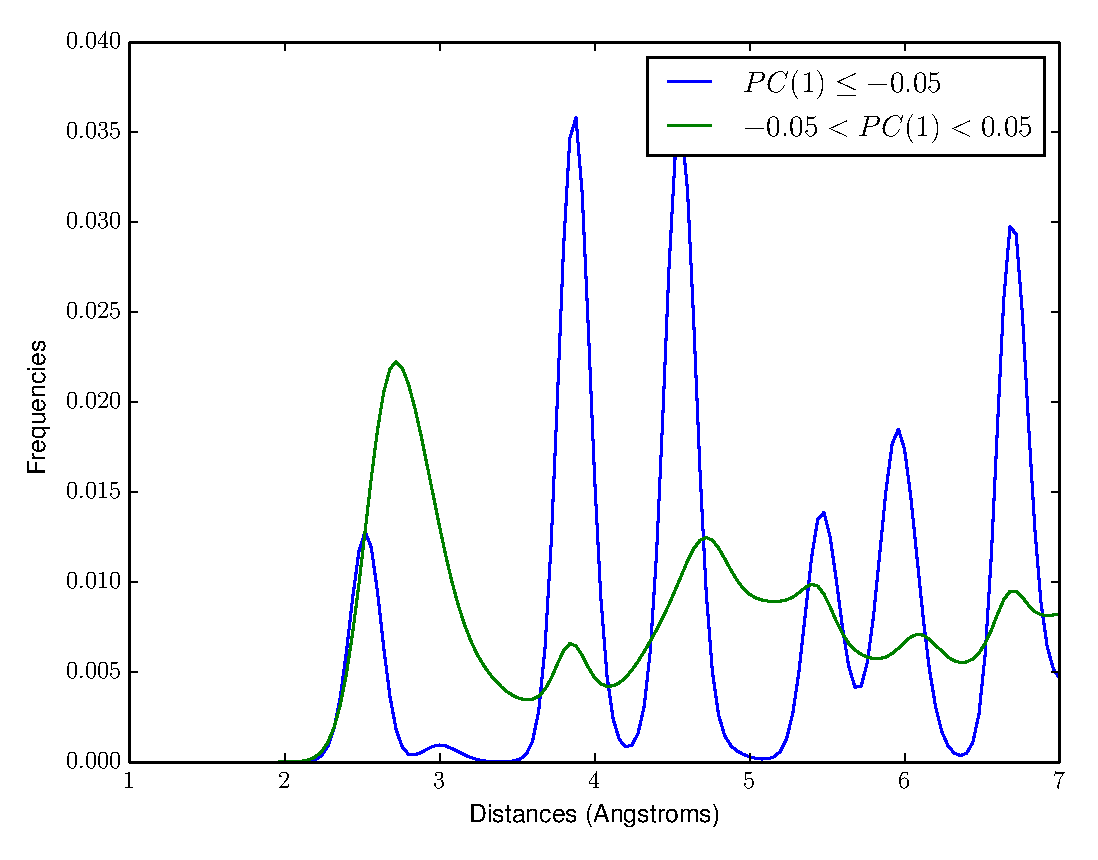
\includegraphics[scale=0.8]{figs/eigenOutlier1.eps}
    \caption{First Principal Component Outliers}
  \end{center}
\end{figure}

\begin{figure}[ht]
  \begin{center}
    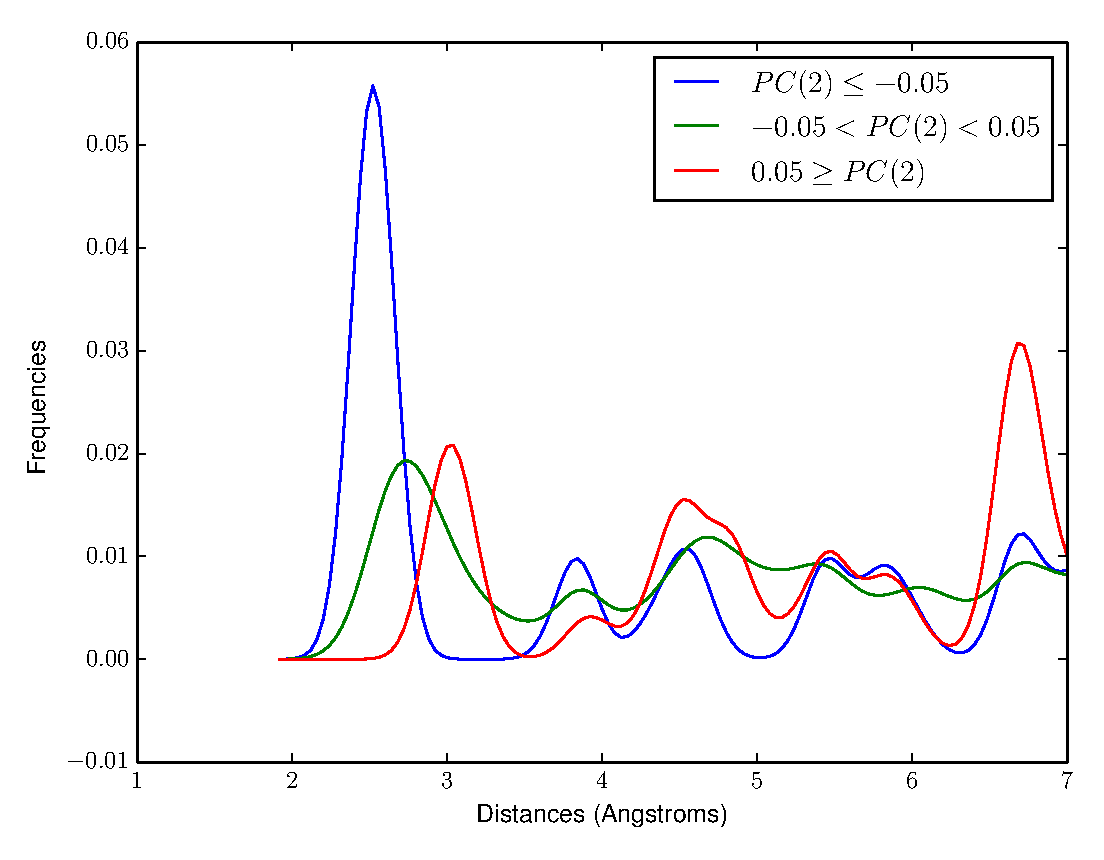
\includegraphics[scale=0.8]{figs/eigenOutlier2.eps}
    \caption{Second Principal Component Outliers}
  \end{center}
\end{figure}

\begin{figure}[ht]
  \begin{center}
    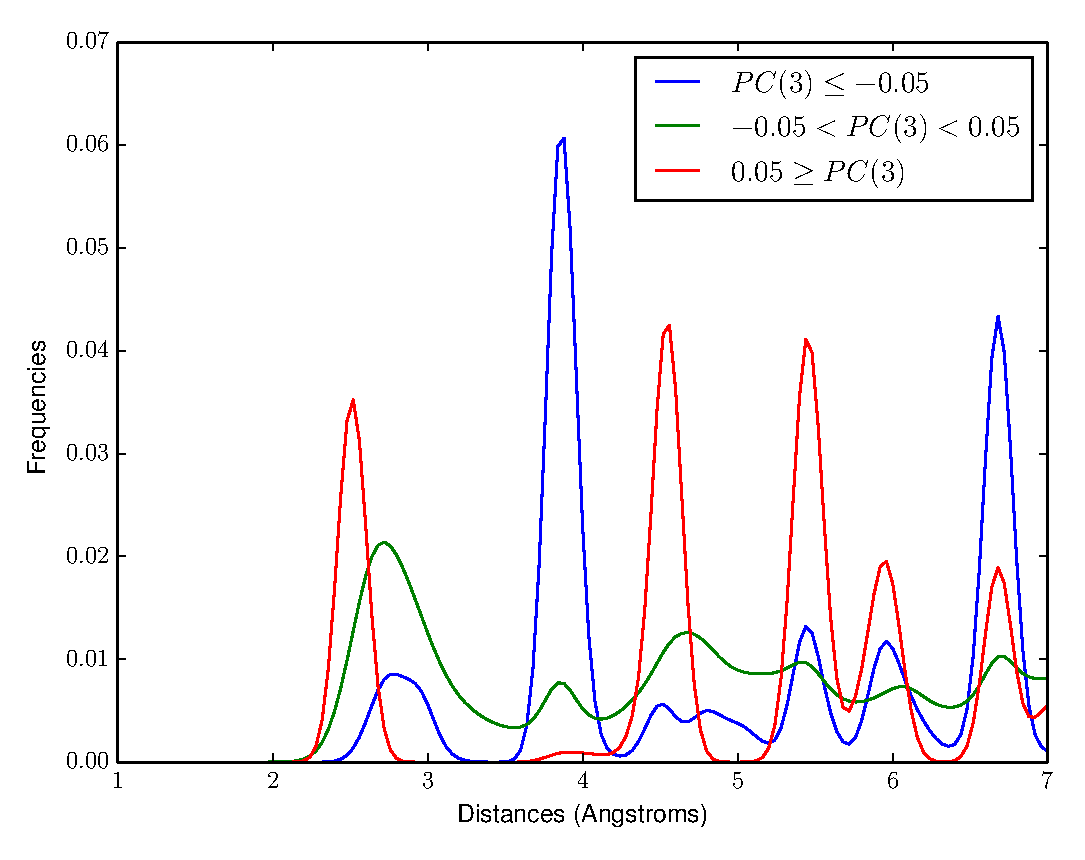
\includegraphics[scale=0.8]{figs/eigenOutlier3.eps}
    \caption{Third Principal Component Outliers}
  \end{center}
\end{figure}

\begin{figure}[ht]
  \begin{center}
    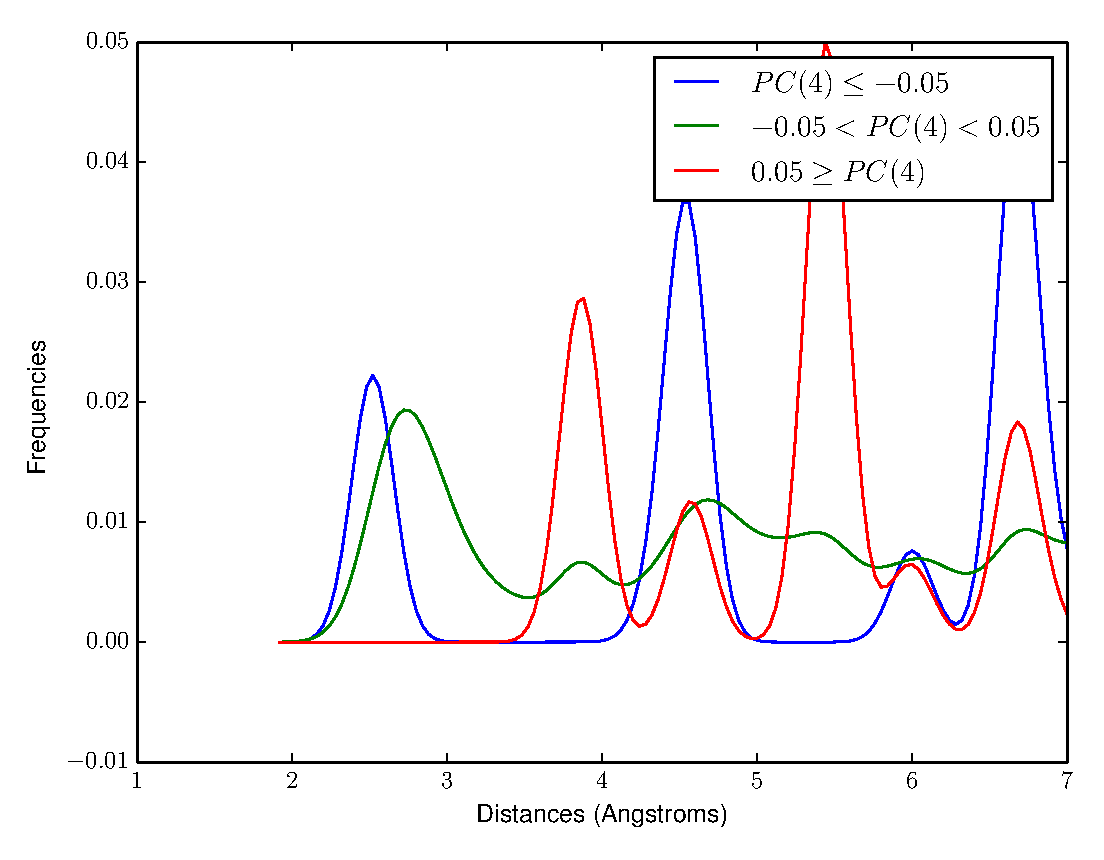
\includegraphics[scale=0.8]{figs/eigenOutlier4.eps}
    \caption{Fourth Principal Component Outliers}
  \end{center}
\end{figure}

\begin{figure}[ht]
  \begin{center}
    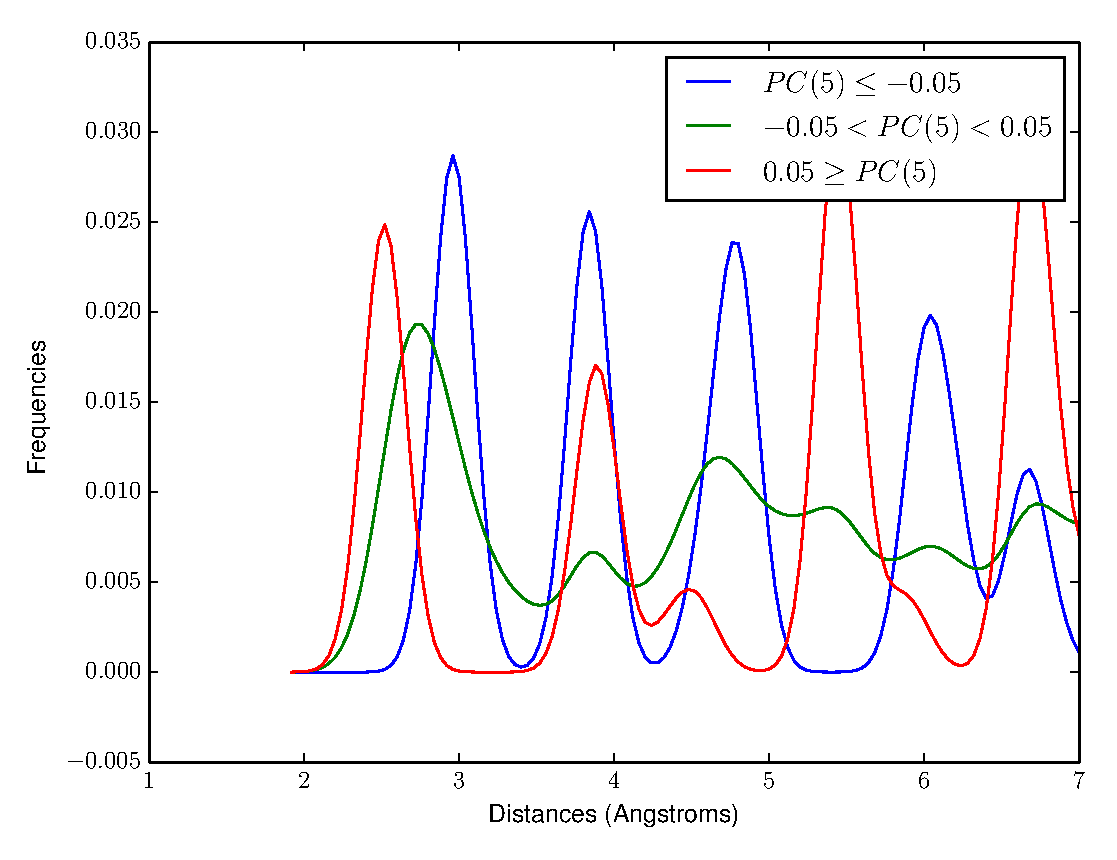
\includegraphics[scale=0.8]{figs/eigenOutlier5.eps}
    \caption{Fifth Principal Component Outliers}
  \end{center}
\end{figure}
\clearpage

\subsection{Experimental Image Recognition}
\subsubsection{3 Principal Components}
\begin{table}[h]
  \begin{center}
\begin{tabular}{|l|l|l|l|l|l|}
\hline
\textbf{Image}     & \textbf{Best Match} & \textbf{2}    & \textbf{3}    & \textbf{4}    & \textbf{5}    \\ \hline
\textbf{ExptGaAs}  & SiLiCalc11436       & SiLiCalc11634 & SiLiCalc11967 & SiLiCalc12738 & SiLiCalc10225 \\ \hline
\textbf{ExptInAs}  & SiLiCalc10643       & SiLiCalc10560 & SiLiCalc10693 & SiLiCalc10617 & SiLiCalc10621 \\ \hline
\textbf{SiLiExpt1} & SiLiCalc10208       & SiLiCalc10315 & SiLiCalc10317 & SiLiCalc10188 & SiLiCalc10187 \\ \hline
\textbf{SiLiExpt2} & SiLiCalc10317       & SiLiCalc10287 & SiLiCalc10320 & SiLiCalc10283 & SiLiCalc10273 \\ \hline
\textbf{SiLiExpt3} & SiLiCalc10287       & SiLiCalc10239 & SiLiCalc10259 & SiLiCalc10317 & SiLiCalc10232 \\ \hline
\textbf{SiLiExpt4} & SiLiCalc10229       & SiLiCalc10225 & SiLiCalc10232 & SiLiCalc10239 & SiLiCalc10259 \\ \hline
\textbf{SiLiExpt5} & SiLiCalc10225       & SiLiCalc10256 & SiLiCalc10232 & SiLiCalc10229 & SiLiCalc10231 \\ \hline
\textbf{SiLiExpt6} & SiLiCalc10322       & SiLiCalc10225 & SiLiCalc10247 & SiLiCalc10229 & SiLiCalc10256 \\ \hline
\textbf{SiLiExpt7} & SiLiCalc10225       & SiLiCalc10322 & SiLiCalc10256 & SiLiCalc10247 & SiLiCalc10229 \\ \hline
\textbf{SiLiExpt8} & SiLiCalc10225       & SiLiCalc10322 & SiLiCalc10247 & SiLiCalc10337 & SiLiCalc10256 \\ \hline
\end{tabular}
  \caption{Recognition with 3 Principal Components}
  \end{center}
\end{table}

\begin{figure}[ht]
  \begin{center}
    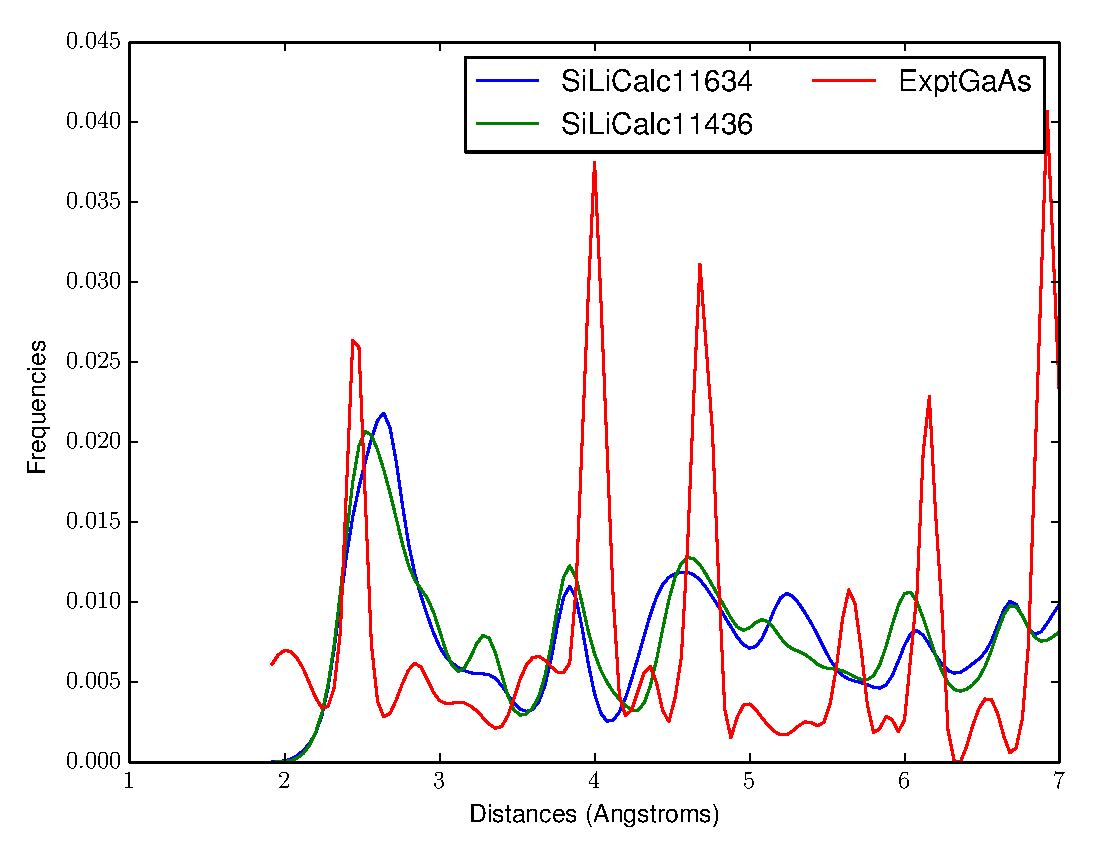
\includegraphics[scale=0.8]{figs/PC3MatchExptGaAs-SiLiCalc11436-SiLiCalc11634.eps}
  \caption{PCA Matches: ExptGaAs, SiLiCalc11436, SiLiCalc11634}
  \end{center}
\end{figure}

\begin{figure}[ht]
  \begin{center}
    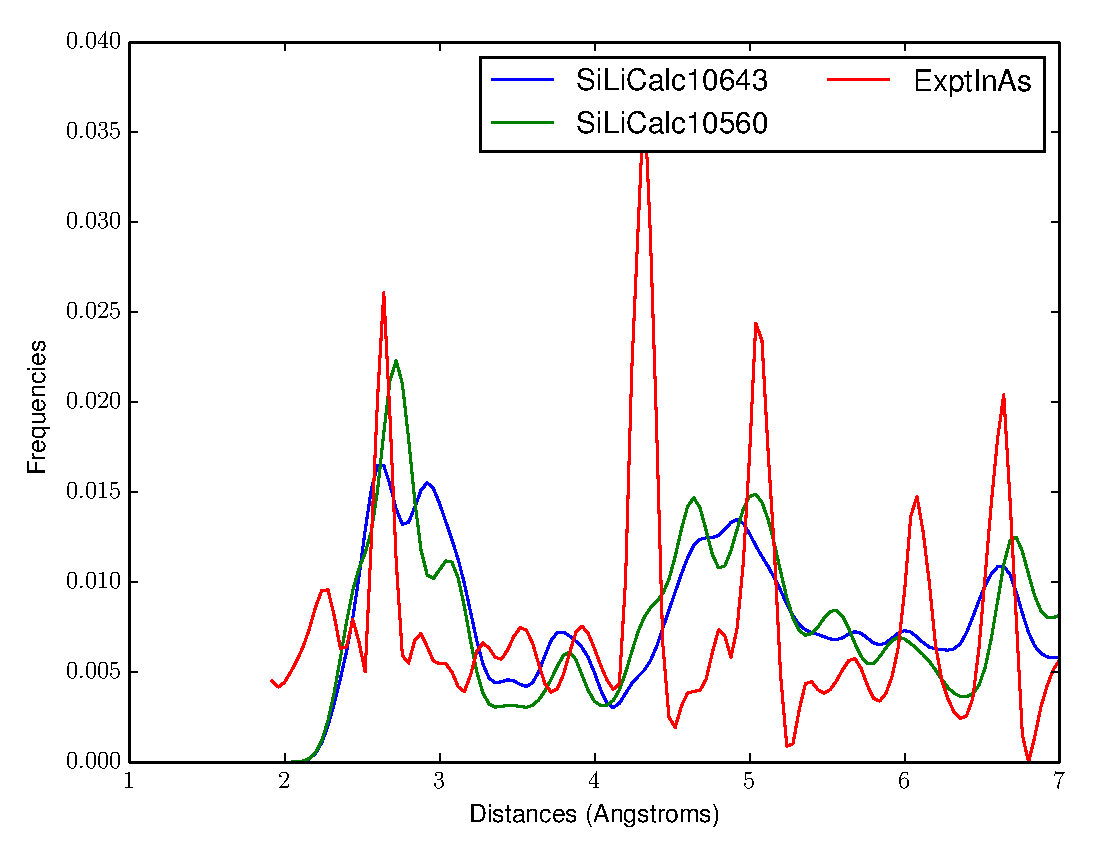
\includegraphics[scale=0.8]{figs/PC3MatchExptInAs-SiLiCalc10643-SiLiCalc10560.eps}
  \caption{PCA Matches: ExptInAs, SiLiCalc10643, SiLiCalc10560}
  \end{center}
\end{figure}

\begin{figure}[ht]
  \begin{center}
    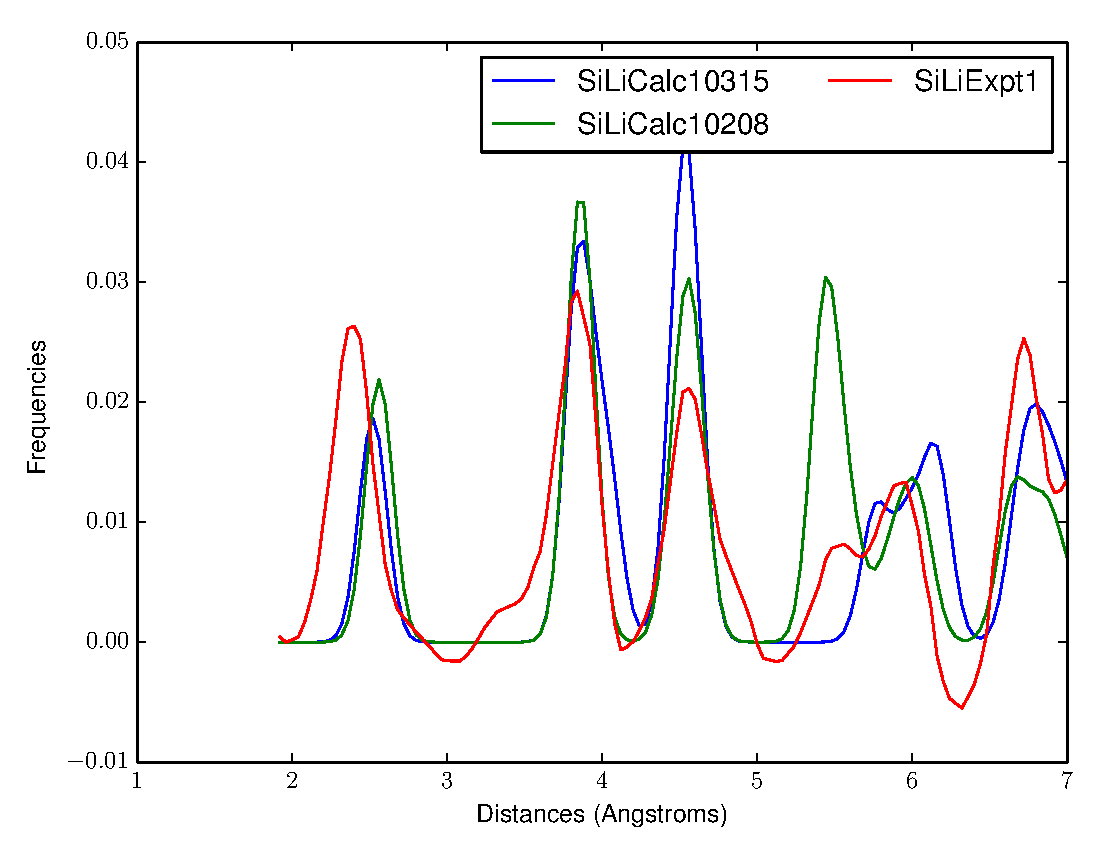
\includegraphics[scale=0.8]{figs/PC3MatchSiLiExpt1-SiLiCalc10208-SiLiCalc10315.eps}
  \caption{PCA Matches: SiLiExpt1, SiLiCalc10208, SiLiCalc10315}
  \end{center}
\end{figure}

\begin{figure}[ht]
  \begin{center}
    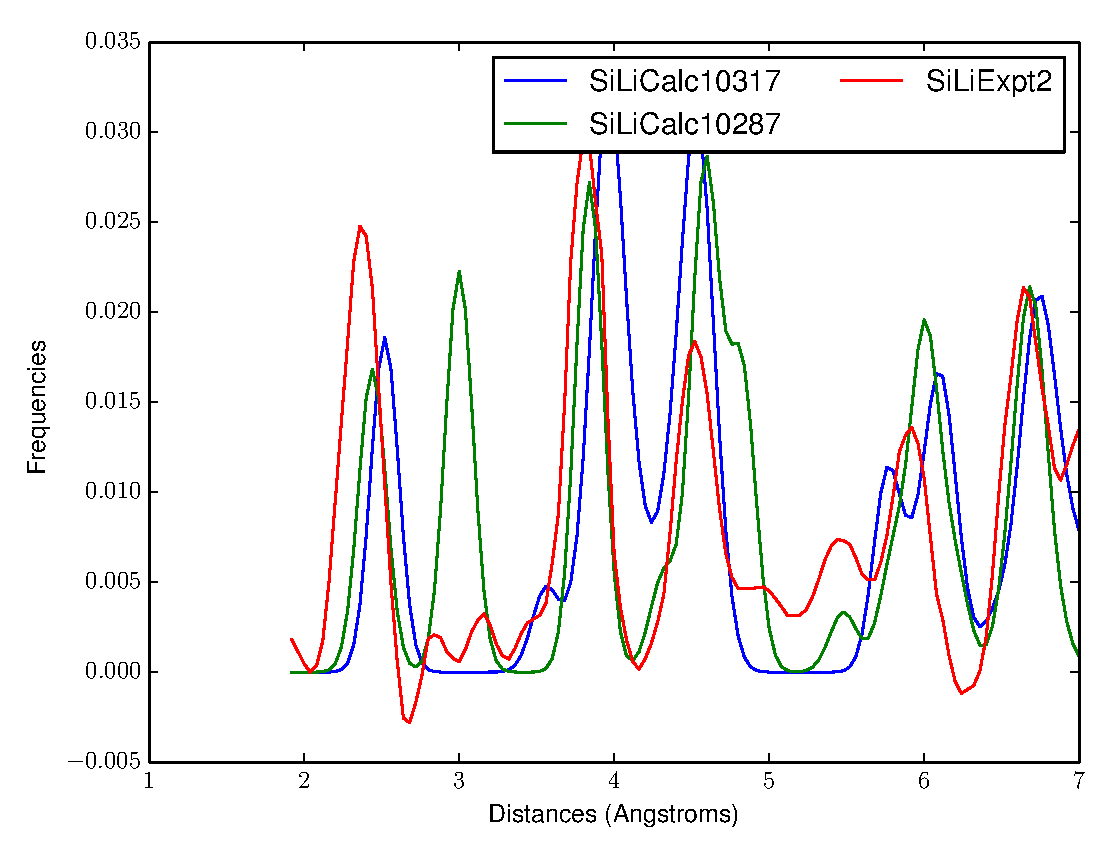
\includegraphics[scale=0.8]{figs/PC3MatchSiLiExpt2-SiLiCalc10317-SiLiCalc10287.eps}
    \caption{PCA Matches: SiLiExpt2, SiLiCalc10317, SiLiCalc10287}
  \end{center}
\end{figure}

\begin{figure}[ht]
  \begin{center}
    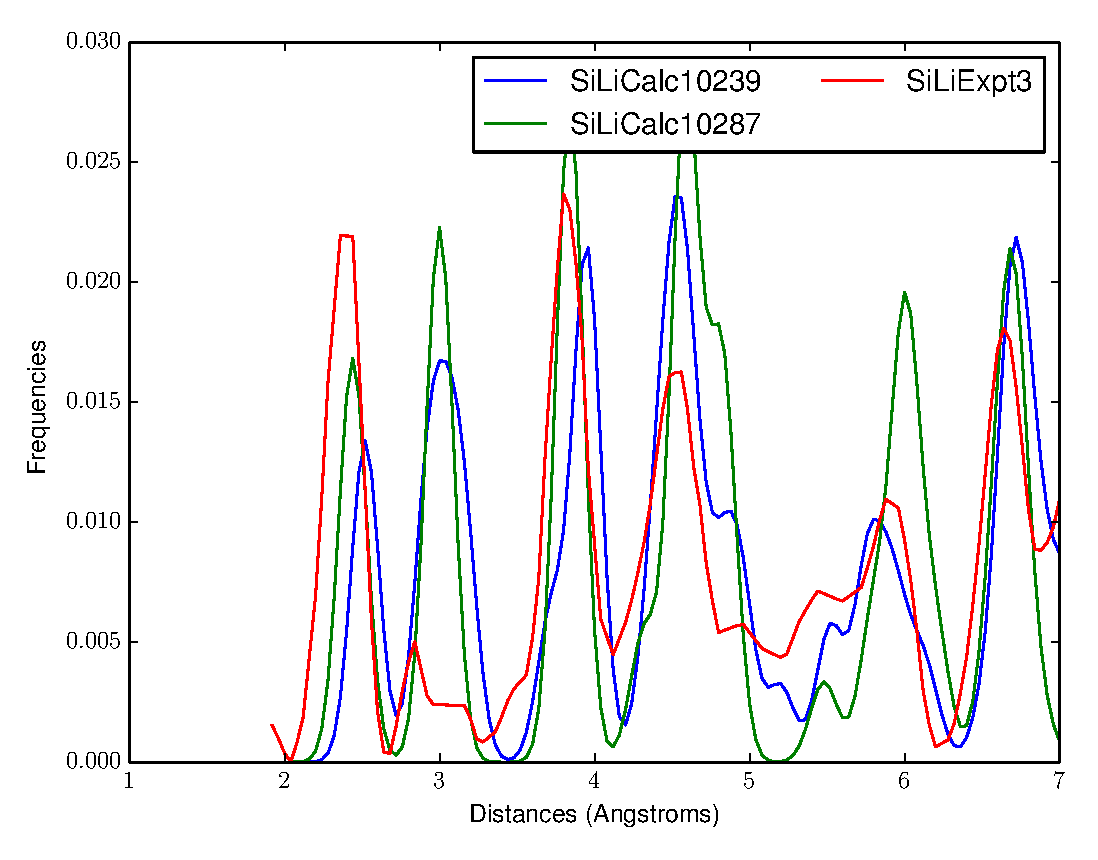
\includegraphics[scale=0.8]{figs/PC3MatchSiLiExpt3-SiLiCalc10287-SiLiCalc10239.eps}
    \caption{PCA Matches: SiLiExpt3, SiLiCalc10287, SiLiCalc10239}
  \end{center}
\end{figure}

\begin{figure}[ht]
  \begin{center}
    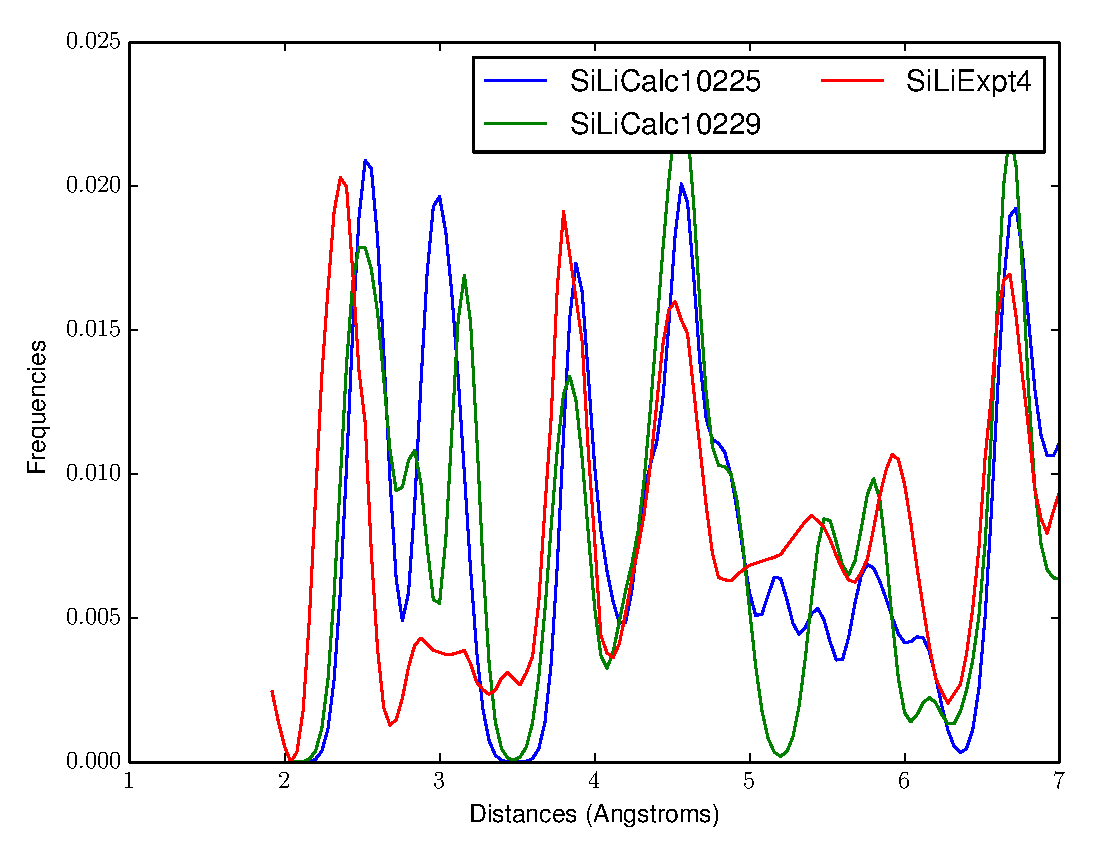
\includegraphics[scale=0.8]{figs/PC3MatchSiLiExpt4-SiLiCalc10229-SiLiCalc10225.eps}
    \caption{PCA Matches: SiLiExpt4, SiLiCalc10229, SiLiCalc10225}
  \end{center}
\end{figure}

\begin{figure}[ht]
  \begin{center}
    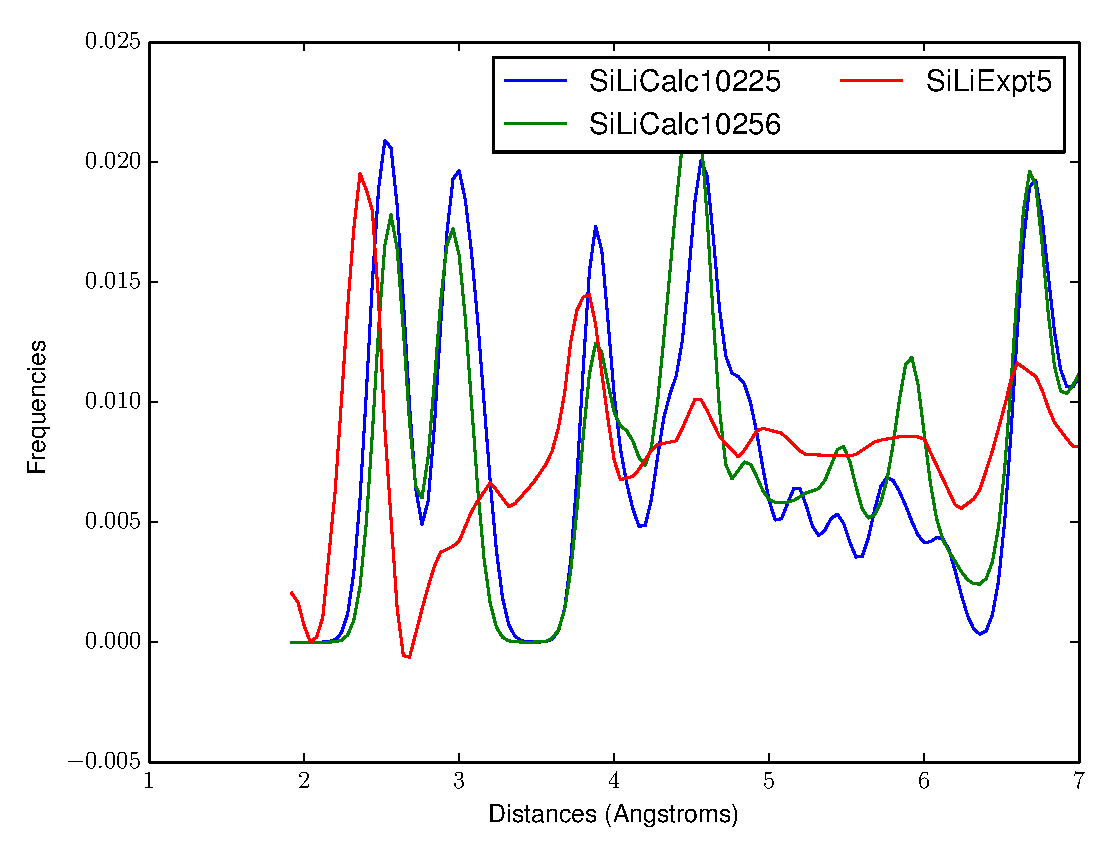
\includegraphics[scale=0.8]{figs/PC3MatchSiLiExpt5-SiLiCalc10225-SiLiCalc10256.eps}
    \caption{PCA Matches: SiLiExpt5, SiLiCalc10225, SiLiCalc10256}
  \end{center}
\end{figure}

\begin{figure}[ht]
  \begin{center}
    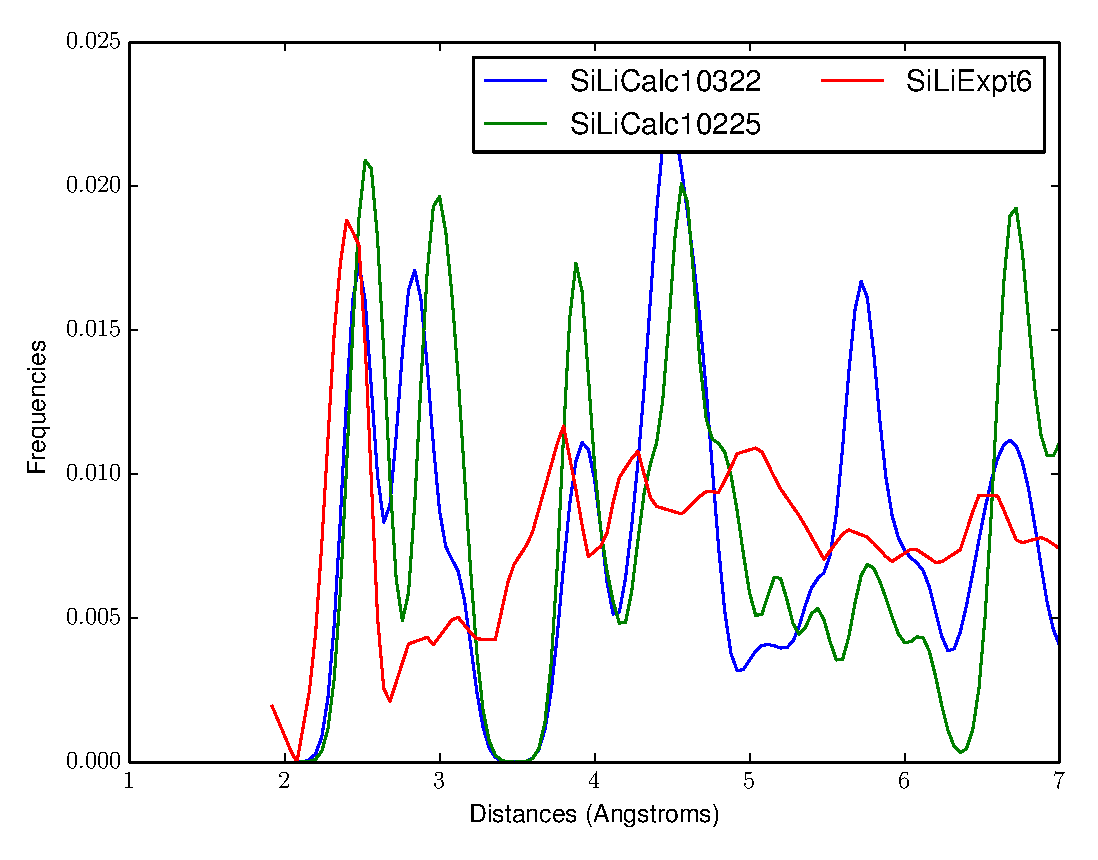
\includegraphics[scale=0.8]{figs/PC3MatchSiLiExpt6-SiLiCalc10322-SiLiCalc10225.eps}
    \caption{PCA Matches: SiLiExpt6, SiLiCalc10322, SiLiCalc10225}
  \end{center}
\end{figure}

\begin{figure}[ht]
  \begin{center}
    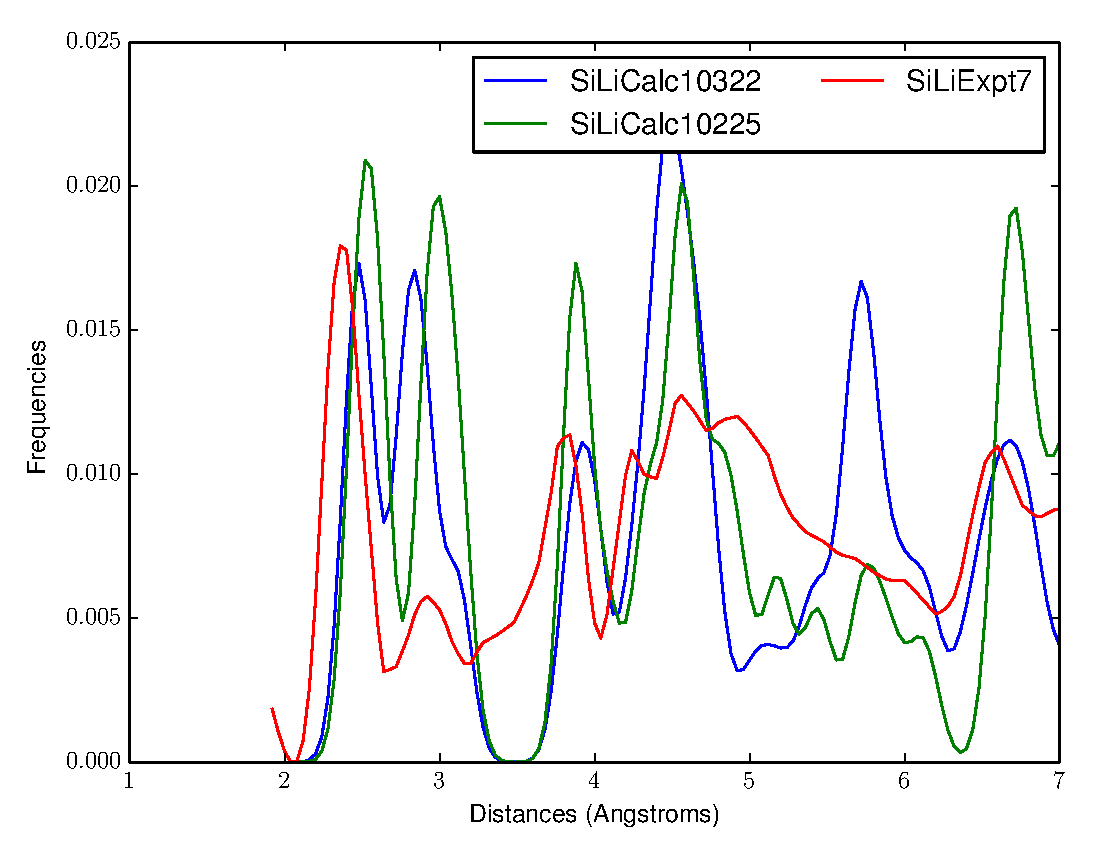
\includegraphics[scale=0.8]{figs/PC3MatchSiLiExpt7-SiLiCalc10225-SiLiCalc10322.eps}
    \caption{PCA Matches: SiLiExpt7, SiLiCalc10225, SiLiCalc10322}
  \end{center}
\end{figure}

\begin{figure}[ht]
  \begin{center}
    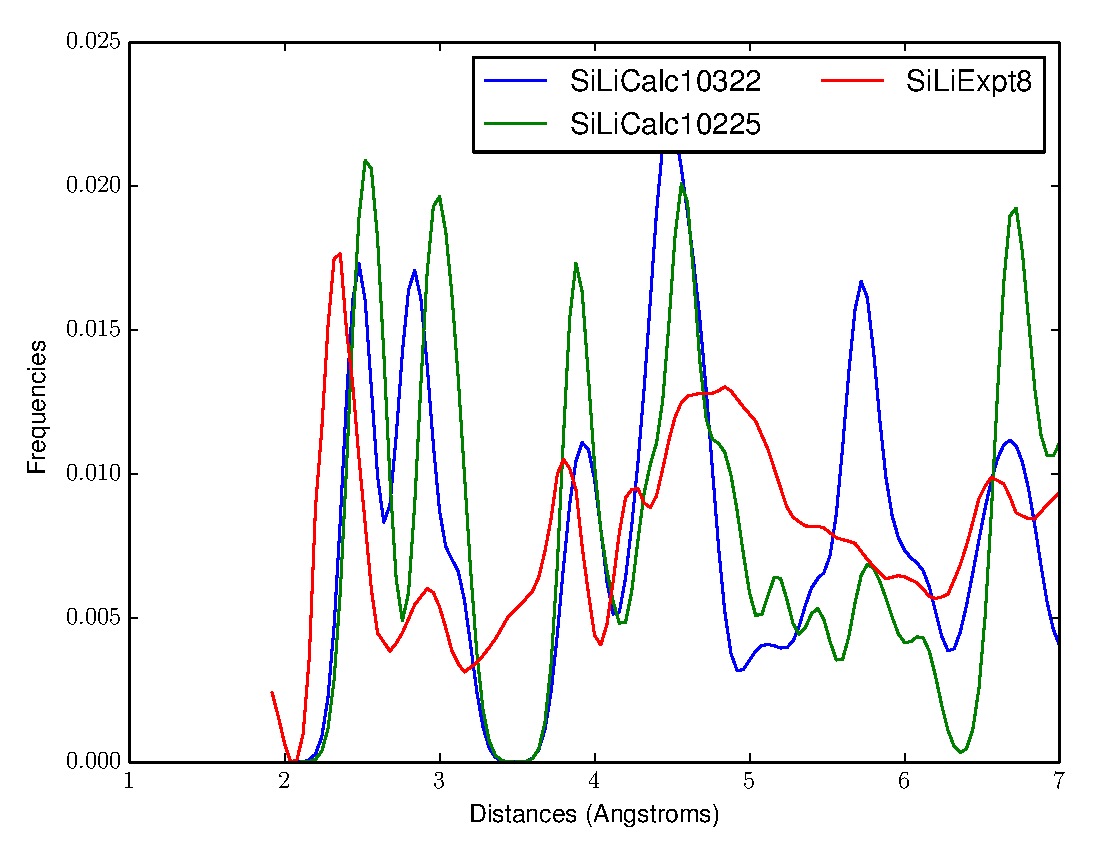
\includegraphics[scale=0.8]{figs/PC3MatchSiLiExpt8-SiLiCalc10225-SiLiCalc10322.eps}
    \caption{PCA Matches: SiLiExpt8, SiLiCalc10225, SiLiCalc10322}
  \end{center}
\end{figure}
\clearpage

\subsubsection{10 Principal Components}
\begin{table}[h]
\begin{center}
\begin{tabular}{|l|l|l|l|l|l|}
\hline
\textbf{Image}     & \textbf{Best Match} & \textbf{2}    & \textbf{3}             & \textbf{4}    & \textbf{5}    \\ \hline
\textbf{ExptGaAs}  & \textbf{CalcGaAs}   & SiLiCalc10329 & SiLiCalc11337          & SiLiCalc11436 & SiLiCalc10571 \\ \hline
\textbf{ExptInAs}  & SiLiCalc10646       & SiLiCalc10805 & SiLiCalc10792          & SiLiCalc10836 & SiLiCalc10767 \\ \hline
\textbf{SiLiExpt1} & SiLiCalc10213       & SiLiCalc10215 & \textbf{SiLiCalc10001} & SiLiCalc10003 & SiLiCalc10313 \\ \hline
\textbf{SiLiExpt2} & SiLiCalc10001       & SiLiCalc10003 & SiLiCalc10209          & SiLiCalc10317 & SiLiCalc10313 \\ \hline
\textbf{SiLiExpt3} & SiLiCalc10257       & SiLiCalc10317 & SiLiCalc10259          & SiLiCalc10258 & SiLiCalc10256 \\ \hline
\textbf{SiLiExpt4} & SiLiCalc10257       & SiLiCalc10258 & SiLiCalc10256          & SiLiCalc10229 & SiLiCalc10232 \\ \hline
\textbf{SiLiExpt5} & SiLiCalc10445       & SiLiCalc10616 & SiLiCalc11436          & SiLiCalc10329 & SiLiCalc11337 \\ \hline
\textbf{SiLiExpt6} & SiLiCalc10445       & SiLiCalc10616 & SiLiCalc11436          & SiLiCalc10693 & SiLiCalc11337 \\ \hline
\textbf{SiLiExpt7} & SiLiCalc10445       & SiLiCalc10693 & SiLiCalc11337          & SiLiCalc10616 & SiLiCalc10482 \\ \hline
\textbf{SiLiExpt8} & SiLiCalc10445       & SiLiCalc10693 & SiLiCalc10329          & SiLiCalc11337 & SiLiCalc10482 \\ \hline
\end{tabular}
  \caption{Recognition with 10 Principal Components}
  \end{center}
\end{table}

\begin{figure}[ht]
  \begin{center}
    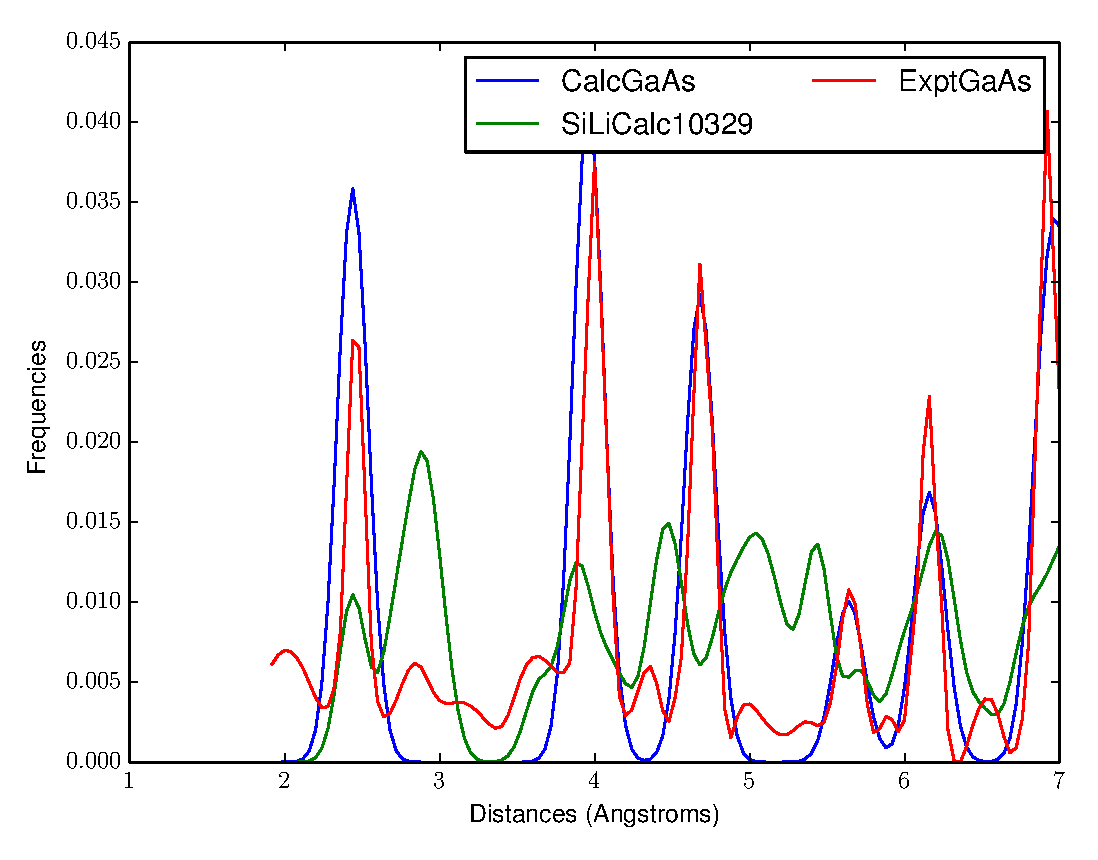
\includegraphics[scale=0.8]{figs/PC10MatchExptGaAs-CalcGaAs-SiLiCalc10329.eps}
    \caption{PCA Matches: ExptGaAs, CalcGaAs, SiLiCalc10329}
  \end{center}
\end{figure}

\begin{figure}[ht]
  \begin{center}
    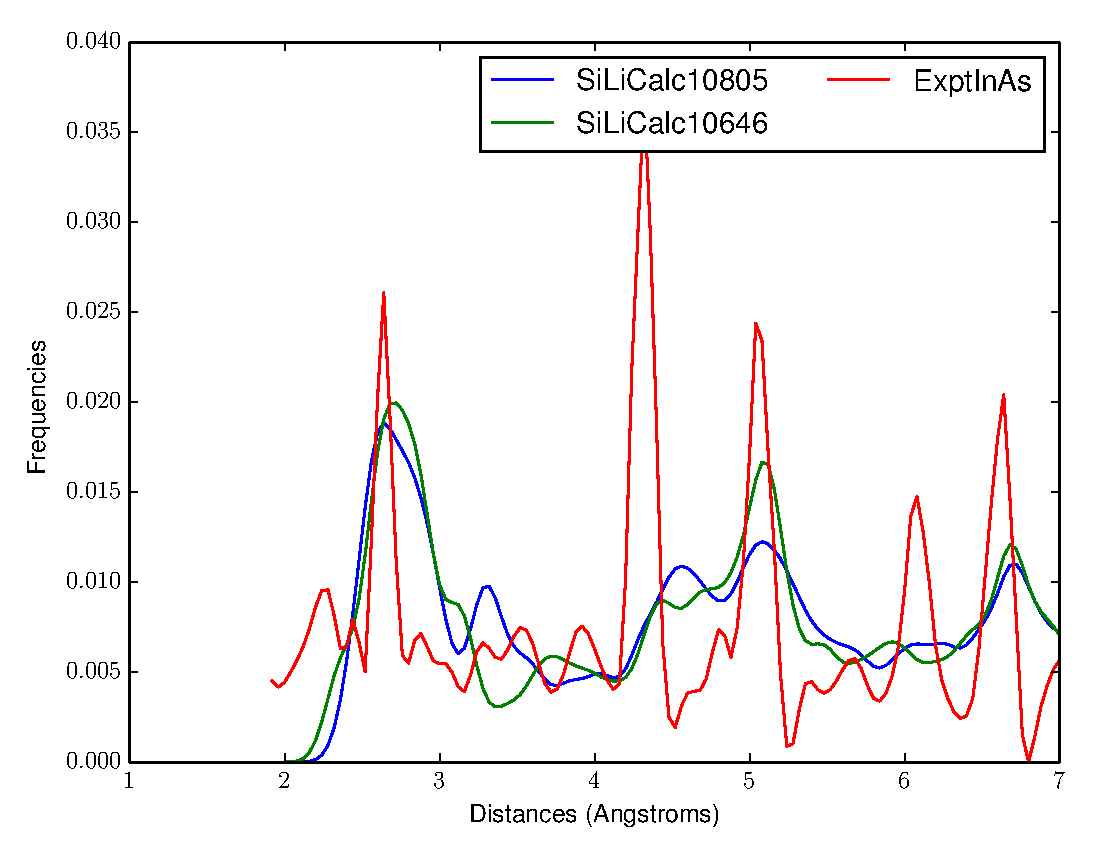
\includegraphics[scale=0.8]{figs/PC10MatchExptInAs-SiLiCalc10646-SiLiCalc10805.eps}
    \caption{PCA Matches: ExptInAs, SiLiCalc10646, SiLiCalc10805}
  \end{center}
\end{figure}

\begin{figure}[ht]
  \begin{center}
    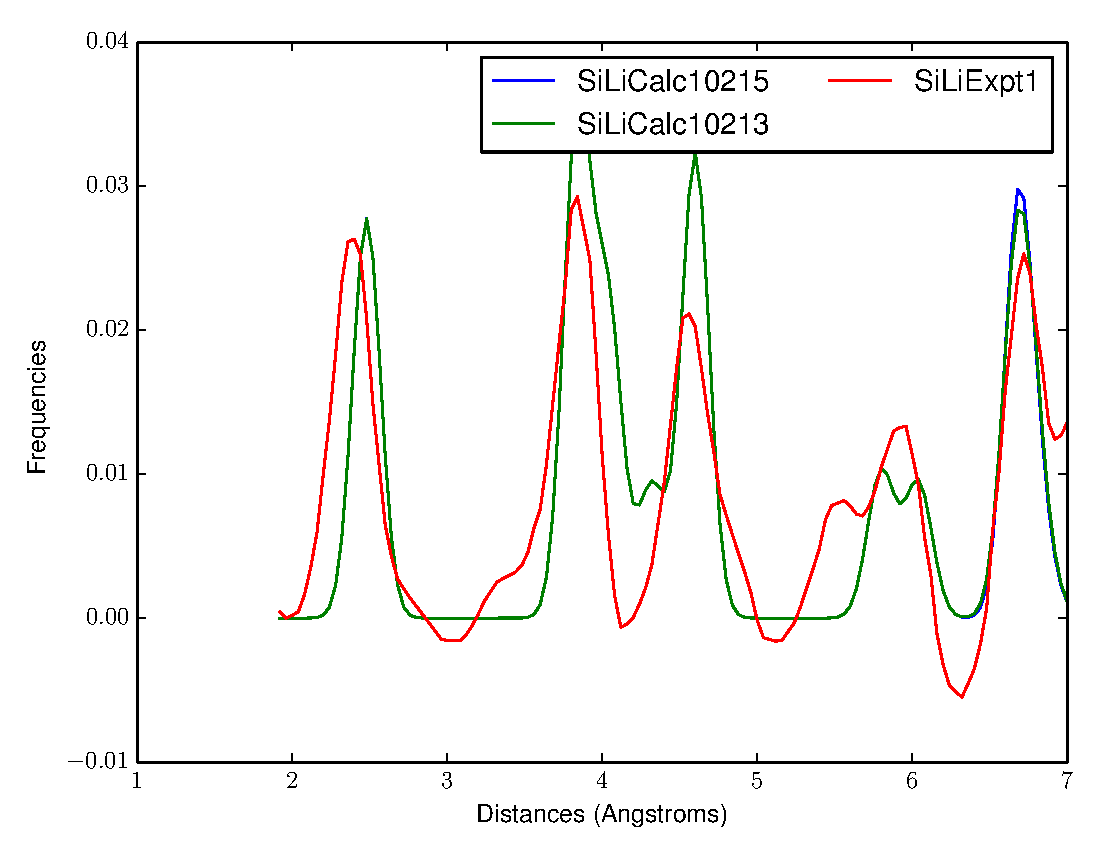
\includegraphics[scale=0.8]{figs/PC10MatchSiLiExpt1-SiLiCalc10213-SiLiCalc10215.eps}
    \caption{PCA Matches: SiLiExpt1, SiLiCalc10213, SiLiCalc10215}
  \end{center}
\end{figure}

\begin{figure}[ht]
  \begin{center}
    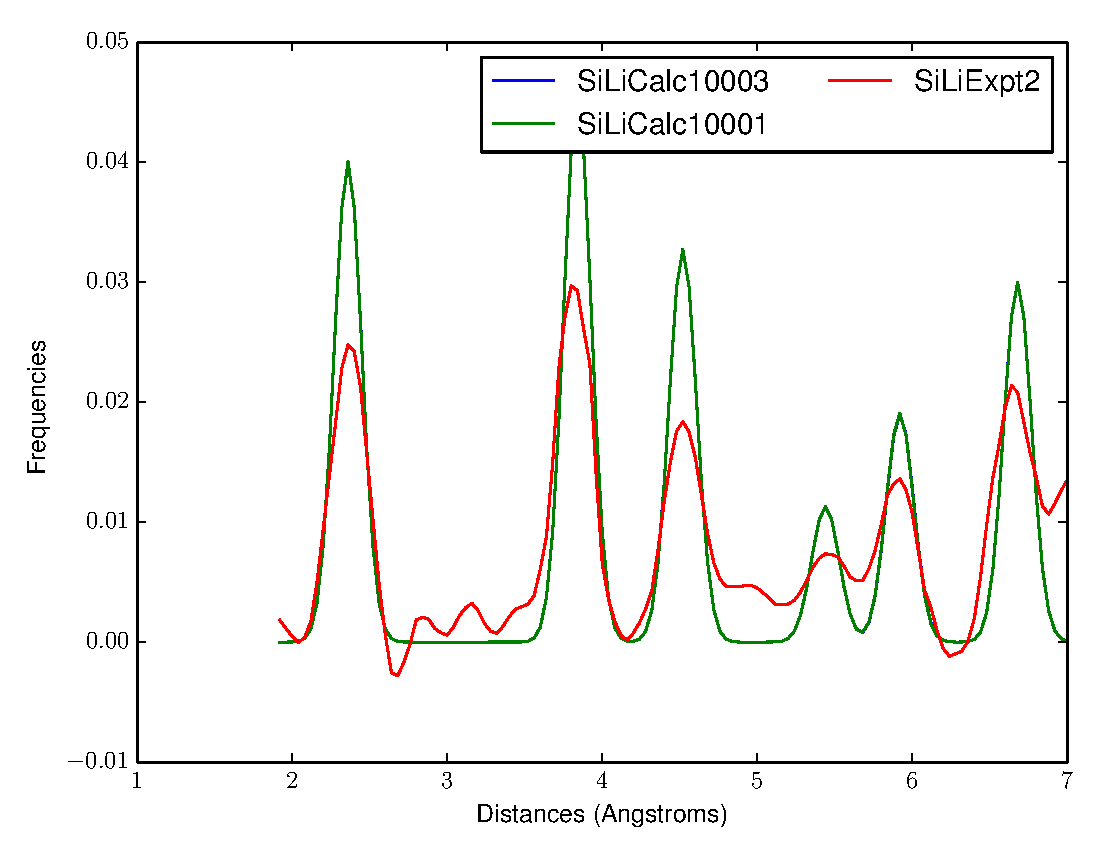
\includegraphics[scale=0.8]{figs/PC10MatchSiLiExpt2-SiLiCalc10001-SiLiCalc10003.eps}
    \caption{PCA Matches: SiLiExpt2, SiLiCalc10001, SiLiCalc10003}
  \end{center}
\end{figure}

\begin{figure}[ht]
  \begin{center}
    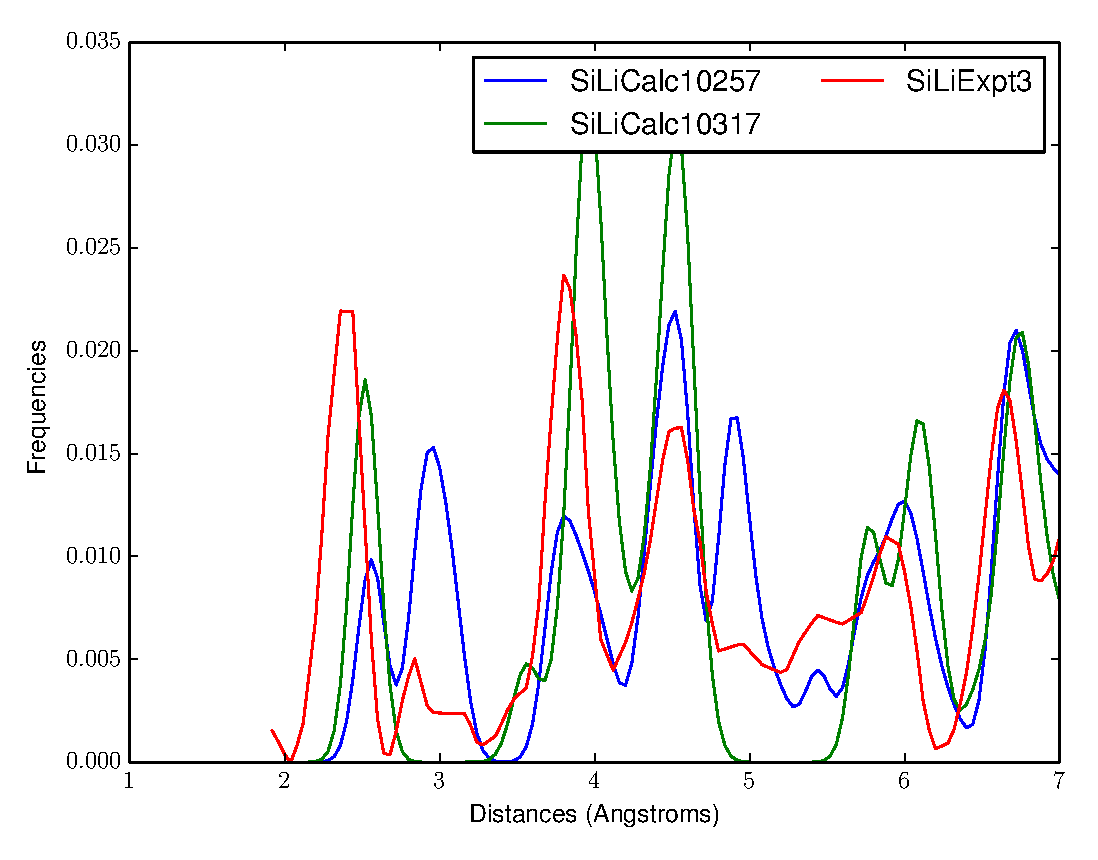
\includegraphics[scale=0.8]{figs/PC10MatchSiLiExpt3-SiLiCalc10257-SiLiCalc10317.eps}
    \caption{PCA Matches: SiLiExpt3, SiLiCalc10257, SiLiCalc10317}
  \end{center}
\end{figure}

\begin{figure}[ht]
  \begin{center}
    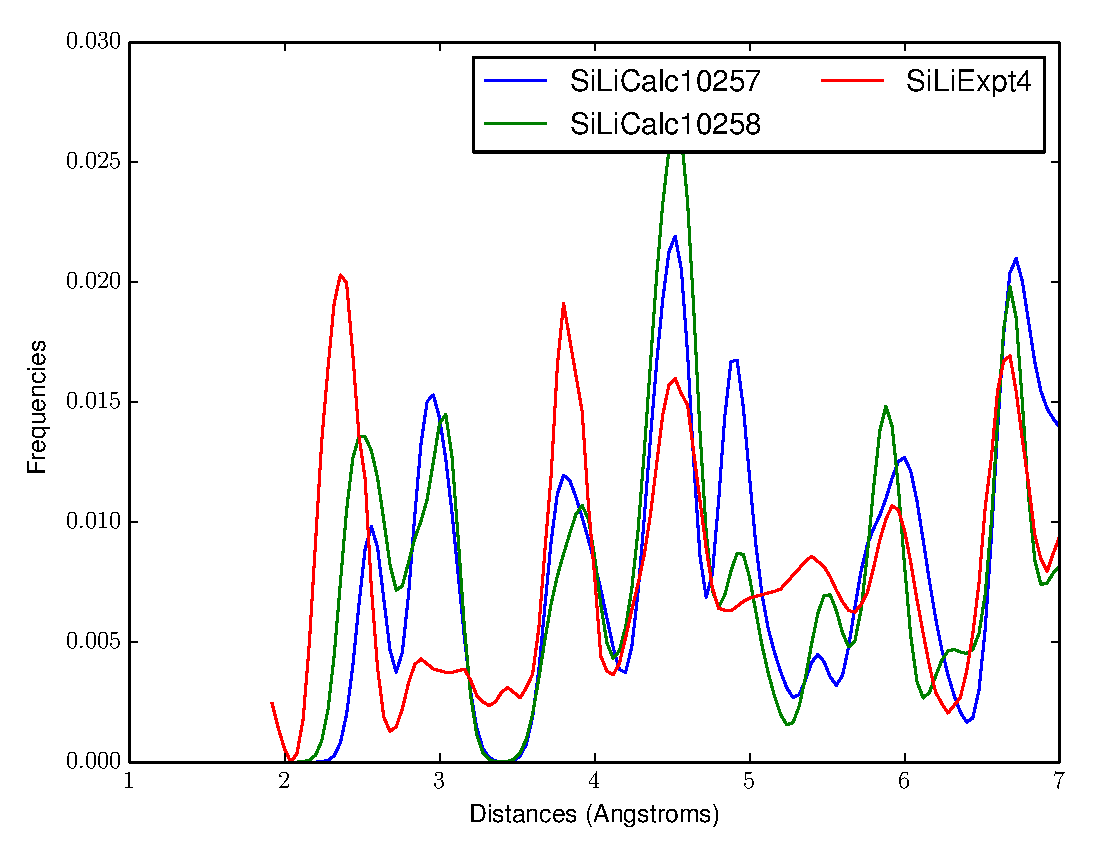
\includegraphics[scale=0.8]{figs/PC10MatchSiLiExpt4-SiLiCalc10257-SiLiCalc10258.eps}
    \caption{PCA Matches: SiLiExpt4, SiLiCalc10257, SiLiCalc10258}
  \end{center}
\end{figure}

\begin{figure}[ht]
  \begin{center}
    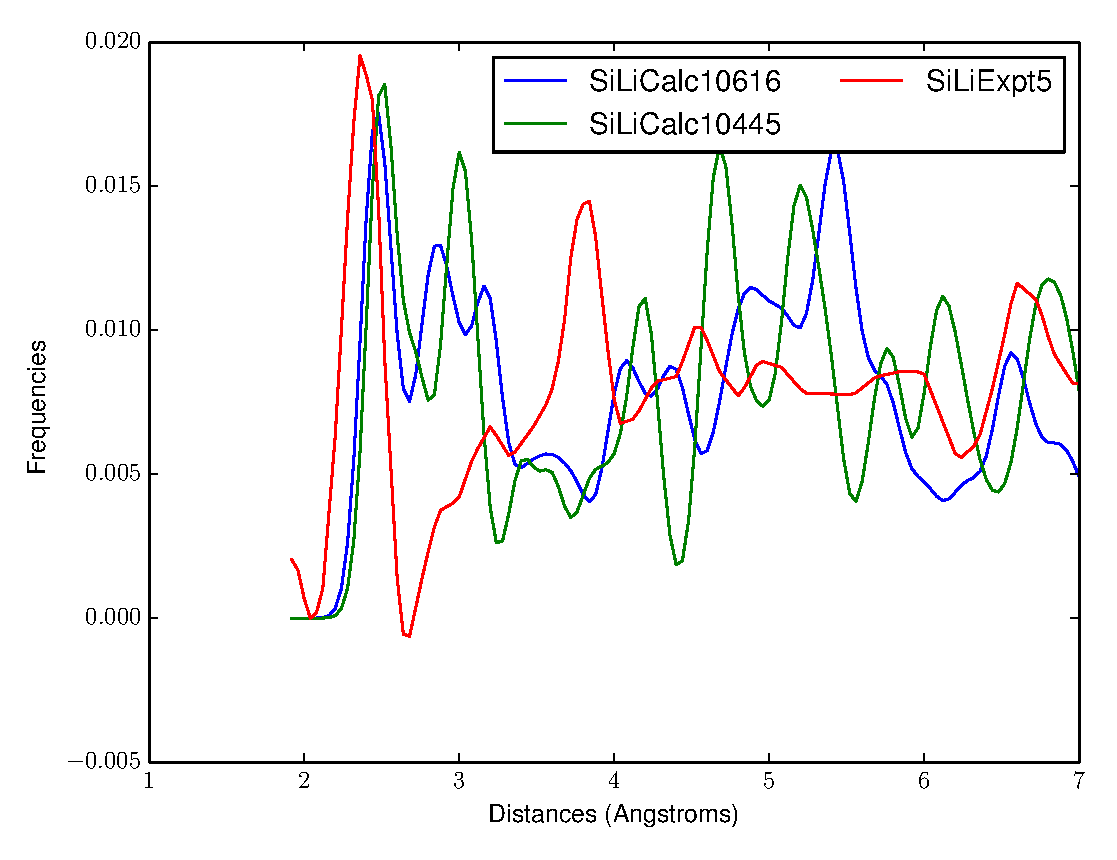
\includegraphics[scale=0.8]{figs/PC10MatchSiLiExpt5-SiLiCalc10445-SiLiCalc10616.eps}
    \caption{PCA Matches: SiLiExpt5, SiLiCalc10445, SiLiCalc10616}
  \end{center}
\end{figure}

\begin{figure}[ht]
  \begin{center}
    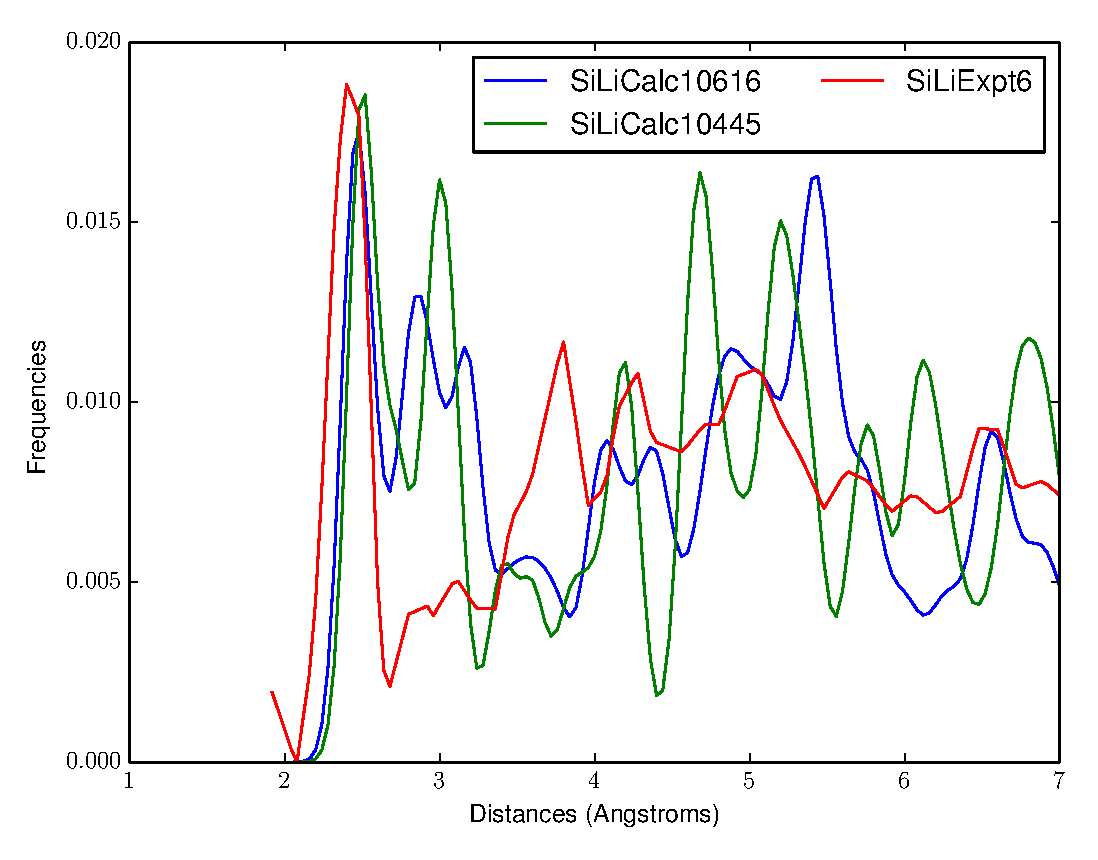
\includegraphics[scale=0.8]{figs/PC10MatchSiLiExpt6-SiLiCalc10445-SiLiCalc10616.eps}
    \caption{PCA Matches: SiLiExpt6, SiLiCalc10445, SiLiCalc10616}
  \end{center}
\end{figure}

\begin{figure}[ht]
  \begin{center}
    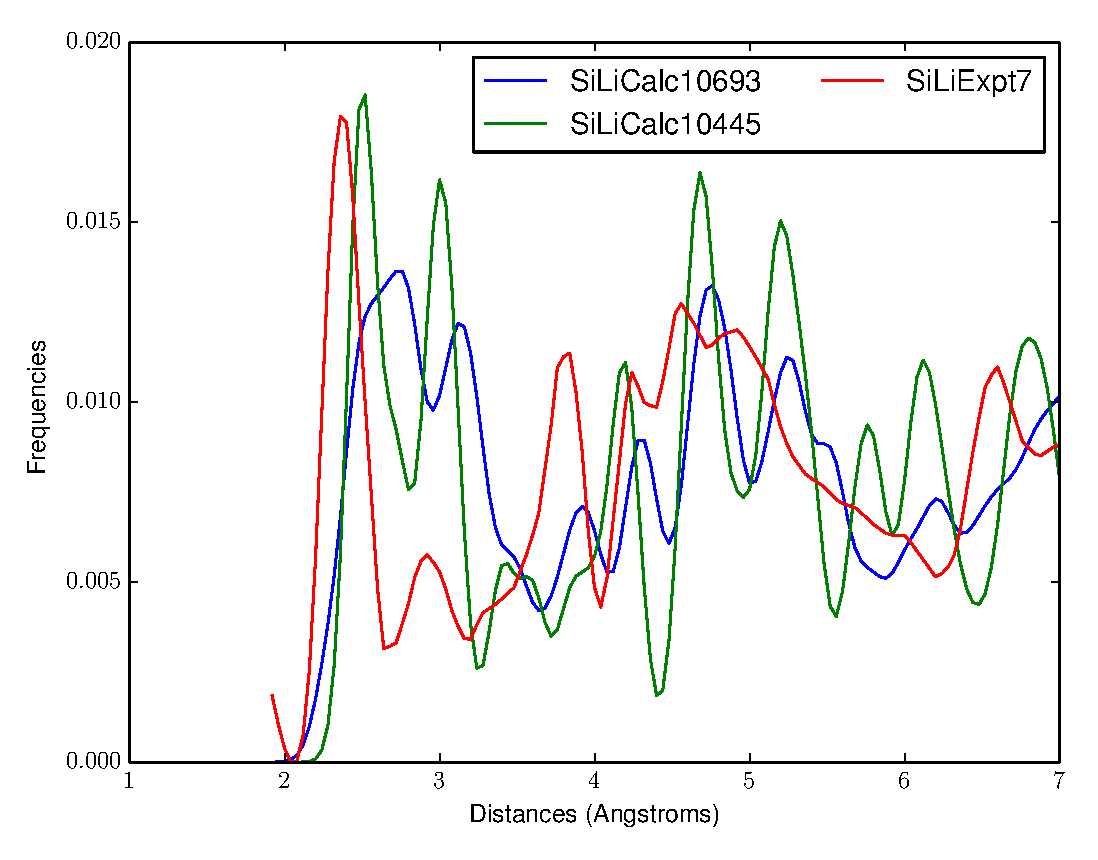
\includegraphics[scale=0.8]{figs/PC10MatchSiLiExpt7-SiLiCalc10445-SiLiCalc10693.eps}
    \caption{PCA Matches: SiLiExpt7, SiLiCalc10445, SiLiCalc10693}
  \end{center}
\end{figure}

\begin{figure}[ht]
  \begin{center}
    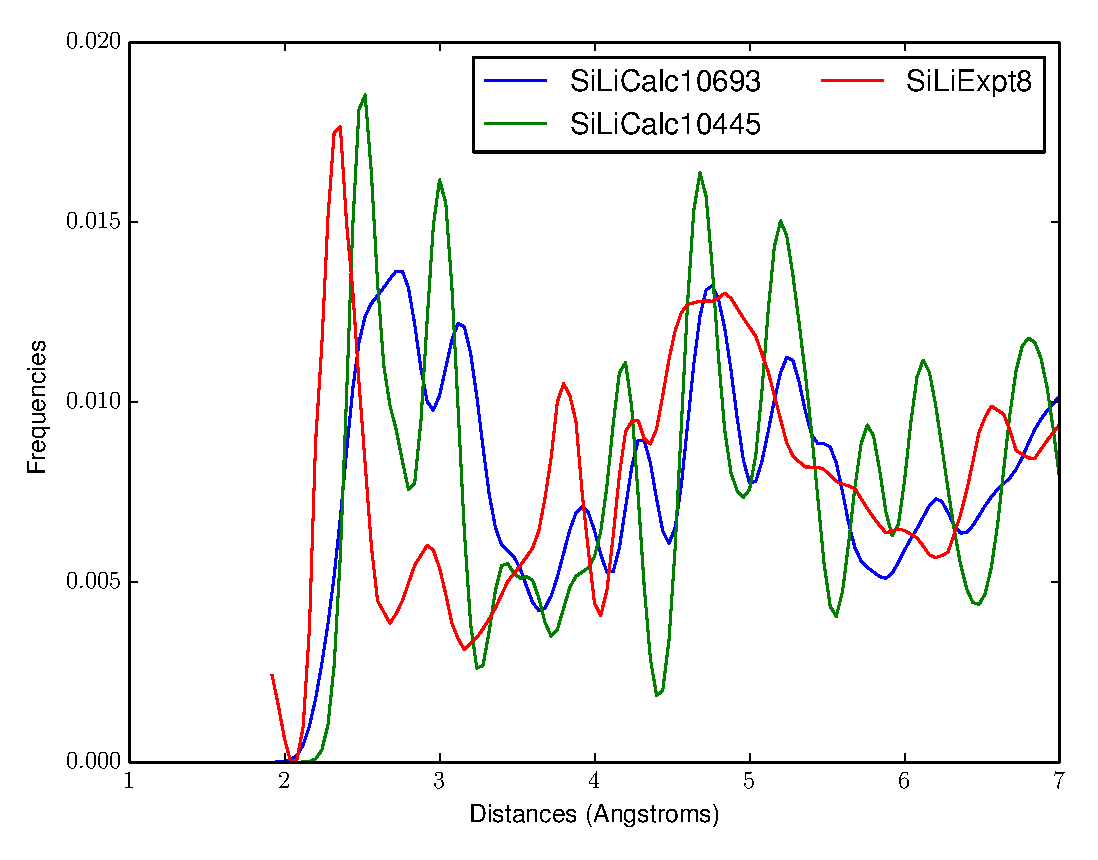
\includegraphics[scale=0.8]{figs/PC10MatchSiLiExpt8-SiLiCalc10445-SiLiCalc10693.eps}
    \caption{PCA Matches: SiLiExpt8, SiLiCalc10445, SiLiCalc10693}
  \end{center}
\end{figure}
\clearpage

\subsubsection{128 Principal Components}
\begin{table}[h]
\begin{tabular}{|l|l|l|l|l|l|}
\hline
\textbf{Image}     & \textbf{Best Match} & \textbf{2}             & \textbf{3}    & \textbf{4}    & \textbf{5}    \\ \hline
\textbf{ExptGaAs}  & \textbf{CalcGaAs}   & SiLiCalc10445          & SiLiCalc11436 & SiLiCalc10693 & SiLiCalc11337 \\ \hline
\textbf{ExptInAs}  & SiLiCalc10429       & SiLiCalc10602          & SiLiCalc10838 & SiLiCalc10901 & SiLiCalc10607 \\ \hline
\textbf{SiLiExpt1} & SiLiCalc10194       & \textbf{SiLiCalc10001} & SiLiCalc10003 & SiLiCalc10136 & SiLiCalc10147 \\ \hline
\textbf{SiLiExpt2} & SiLiCalc10001       & SiLiCalc10003          & SiLiCalc10194 & SiLiCalc10136 & SiLiCalc10147 \\ \hline
\textbf{SiLiExpt3} & SiLiCalc10258       & SiLiCalc10229          & SiLiCalc10245 & SiLiCalc11436 & SiLiCalc10259 \\ \hline
\textbf{SiLiExpt4} & SiLiCalc10258       & SiLiCalc11436          & SiLiCalc10229 & SiLiCalc11337 & SiLiCalc11634 \\ \hline
\textbf{SiLiExpt5} & SiLiCalc10616       & SiLiCalc11337          & SiLiCalc10693 & SiLiCalc11436 & SiLiCalc11336 \\ \hline
\textbf{SiLiExpt6} & SiLiCalc10616       & SiLiCalc10693          & SiLiCalc11337 & SiLiCalc11436 & SiLiCalc11336 \\ \hline
\textbf{SiLiExpt7} & SiLiCalc10693       & SiLiCalc11337          & SiLiCalc10482 & SiLiCalc10616 & SiLiCalc10651 \\ \hline
\textbf{SiLiExpt8} & SiLiCalc10693       & SiLiCalc10651          & SiLiCalc11337 & SiLiCalc10482 & SiLiCalc10616 \\ \hline
\end{tabular}
  \caption{Recognition with 128 Principal Components}
\end{table}

\begin{figure}[ht]
\begin{center}
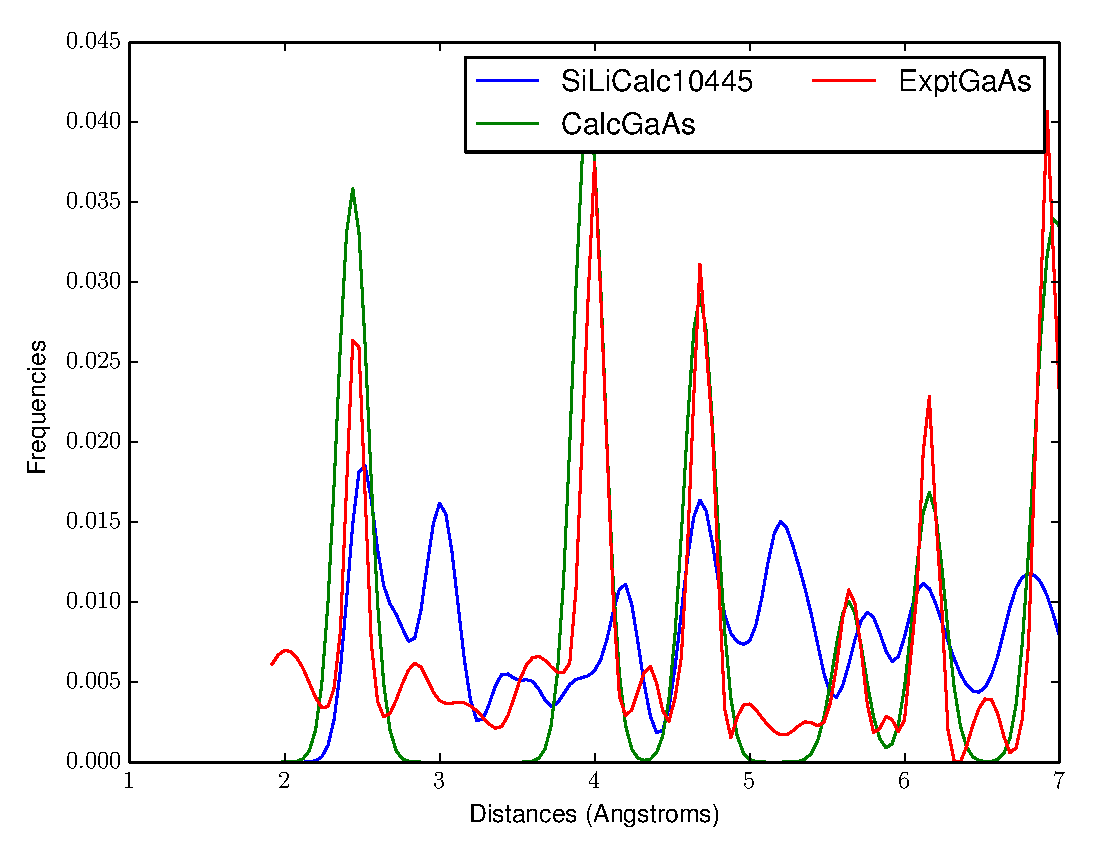
\includegraphics[scale=0.8]{figs/PC128MatchExptGaAs-CalcGaAs-SiLiCalc10445.eps}
\caption{PCA Matches: ExptGaAs, CalcGaAs, SiLiCalc10445}
\end{center}
\end{figure}

\begin{figure}[ht]
\begin{center}
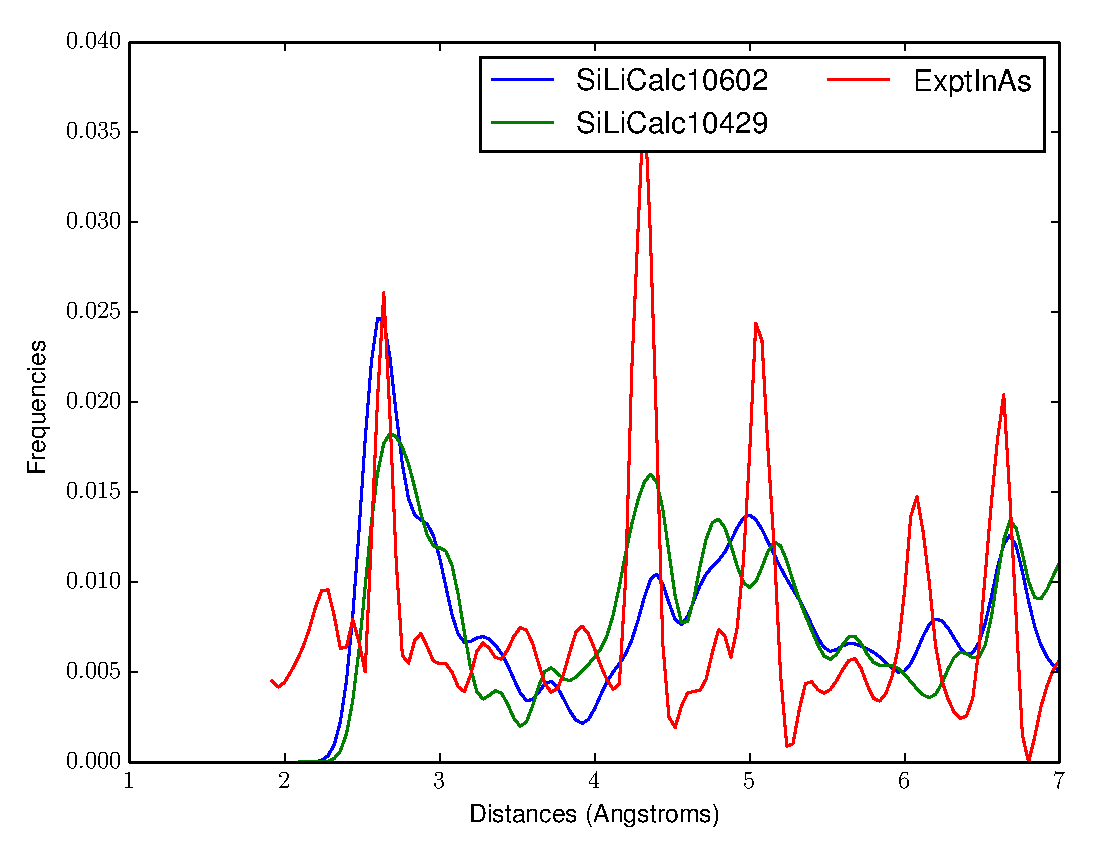
\includegraphics[scale=0.8]{figs/PC128MatchExptInAs-SiLiCalc10429-SiLiCalc10602.eps}
\caption{PCA Matches: ExptInAs, SiLiCalc10429, SiLiCalc10602}
\end{center}
\end{figure}

\begin{figure}[ht]
\begin{center}
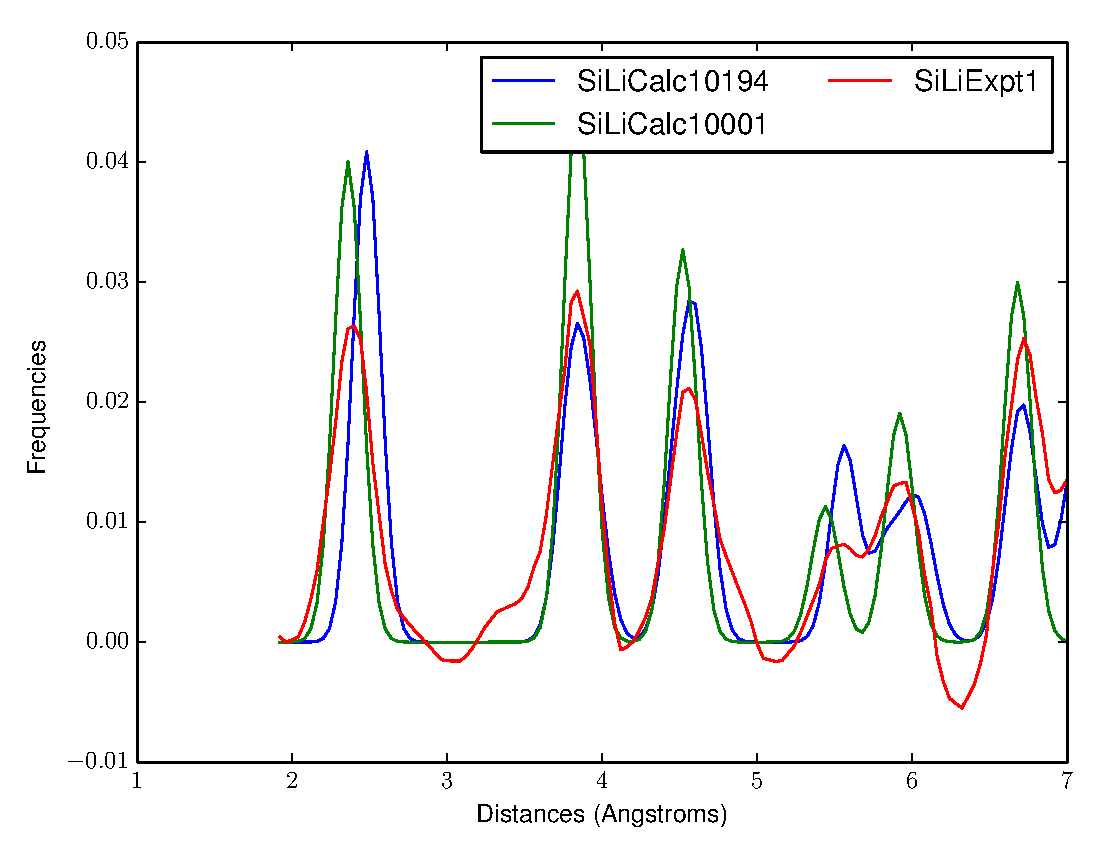
\includegraphics[scale=0.8]{figs/PC128MatchSiLiExpt1-SiLiCalc10194-SiLiCalc10001.eps}
\caption{PCA Matches: SiLiExpt1, SiLiCalc10194, SiLiCalc10001}
\end{center}
\end{figure}

\begin{figure}[ht]
\begin{center}
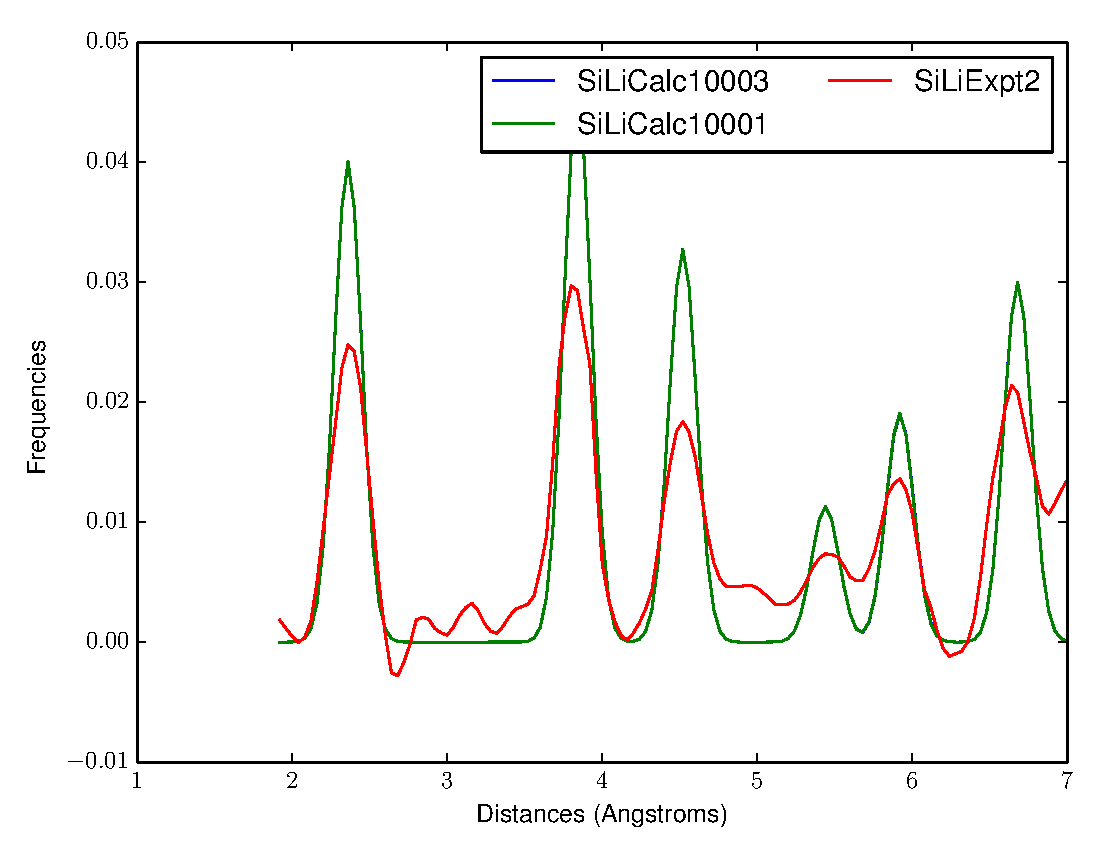
\includegraphics[scale=0.8]{figs/PC128MatchSiLiExpt2-SiLiCalc10001-SiLiCalc10003.eps}
\caption{PCA Matches: SiLiExpt2, SiLiCalc10001, SiLiCalc10003}
\end{center}
\end{figure}

\begin{figure}[ht]
\begin{center}
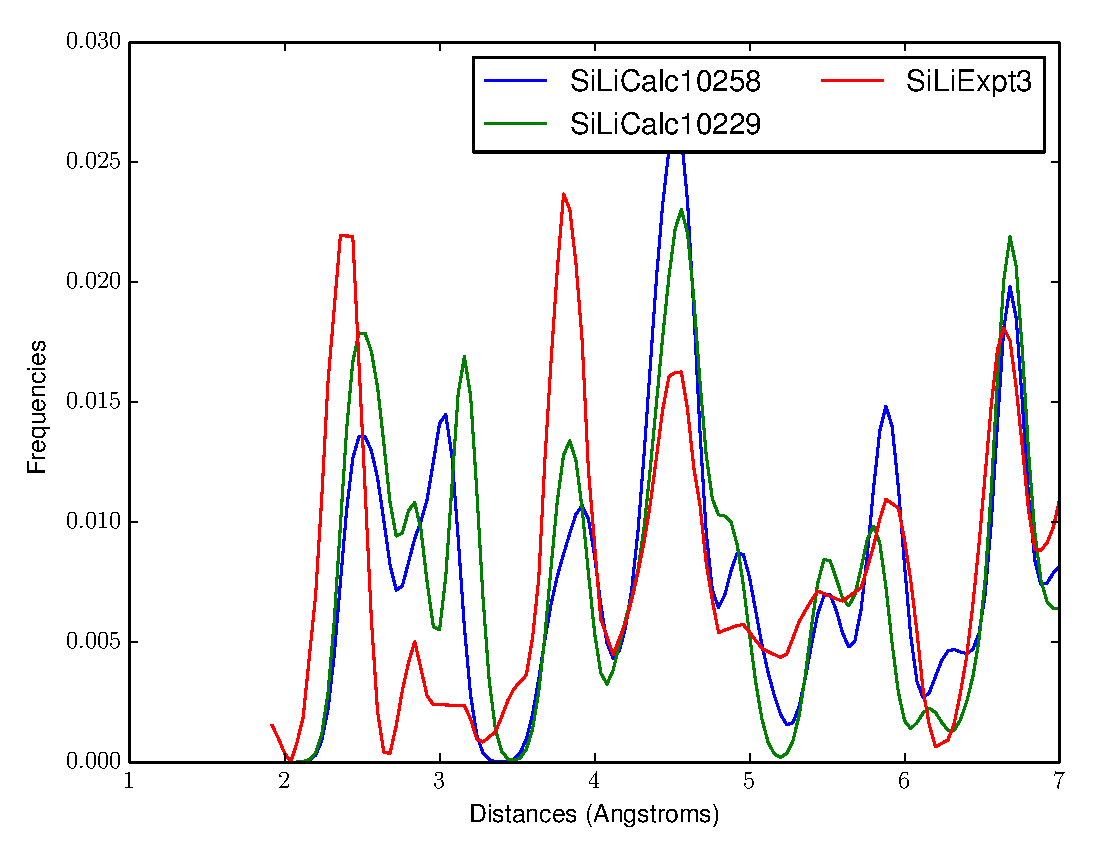
\includegraphics[scale=0.8]{figs/PC128MatchSiLiExpt3-SiLiCalc10258-SiLiCalc10229.eps}
\caption{PCA Matches: SiLiExpt3, SiLiCalc10258, SiLiCalc10229}
\end{center}
\end{figure}

\begin{figure}[ht]
\begin{center}
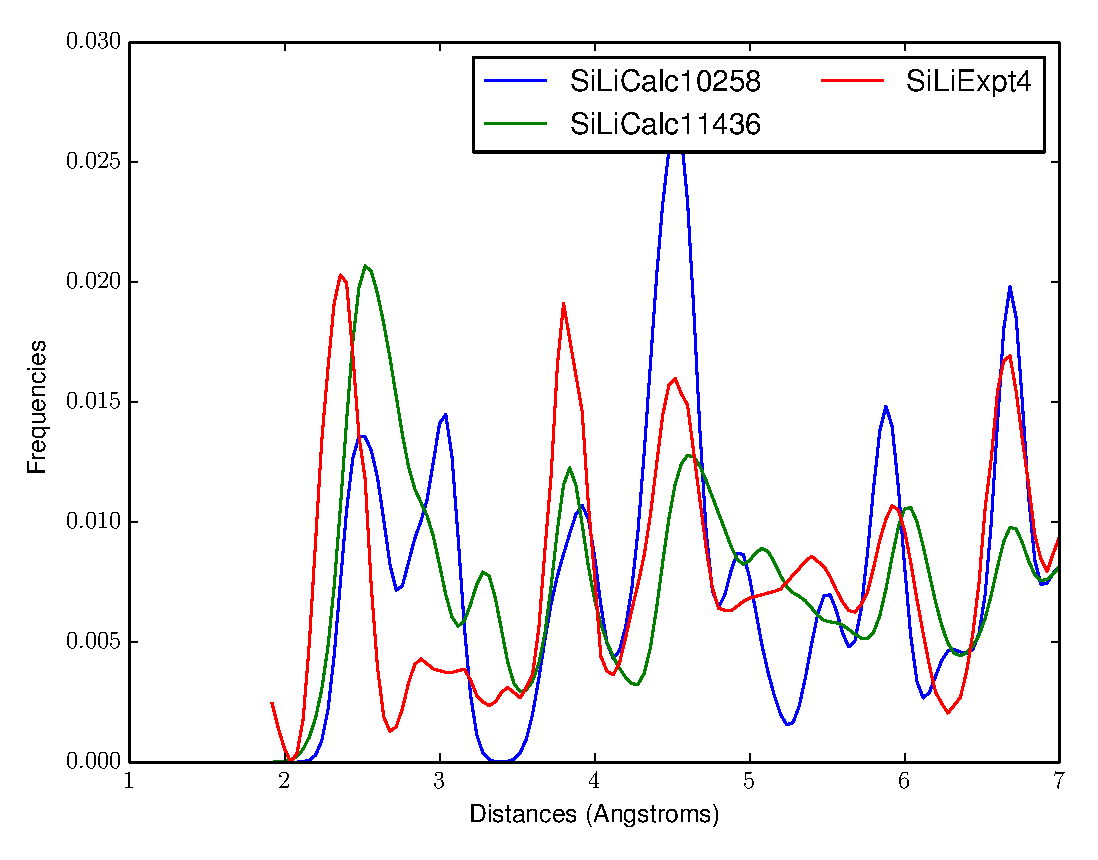
\includegraphics[scale=0.8]{figs/PC128MatchSiLiExpt4-SiLiCalc10258-SiLiCalc11436.eps}
\caption{PCA Matches: SiLiExpt4, SiLiCalc10258, SiLiCalc11436}
\end{center}
\end{figure}

\begin{figure}[ht]
\begin{center}
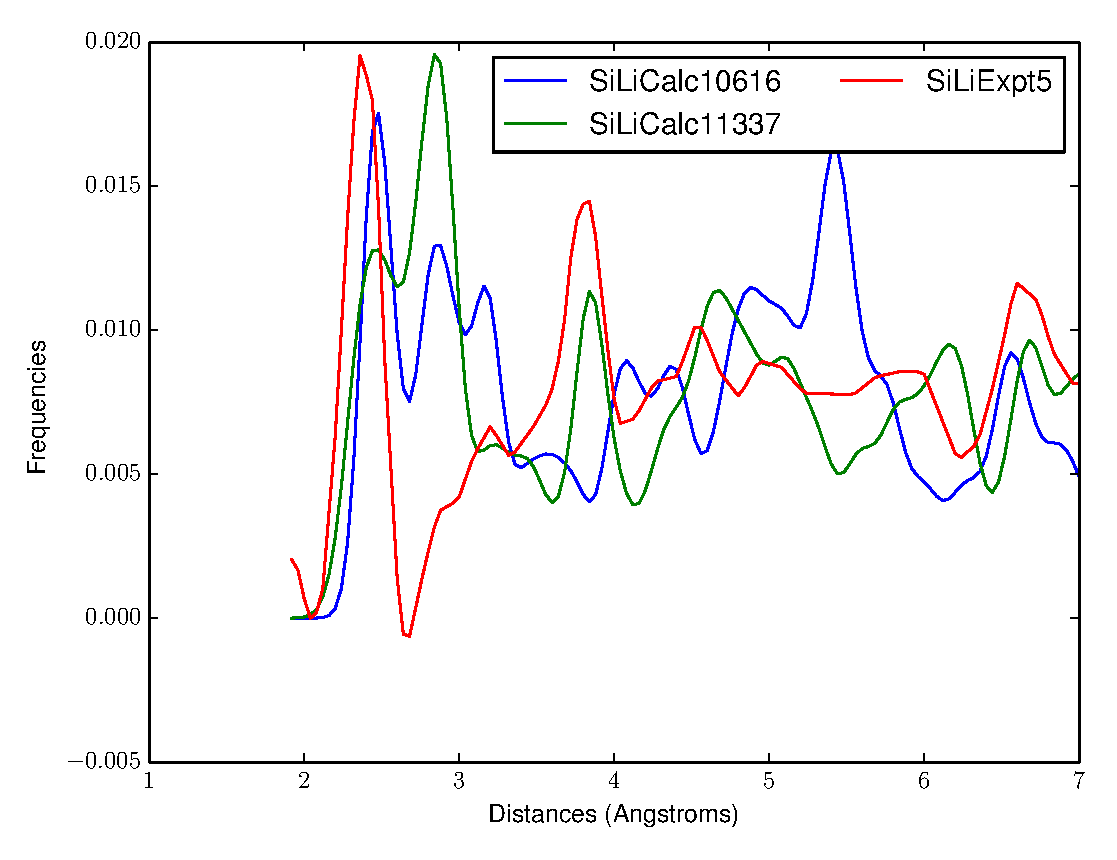
\includegraphics[scale=0.8]{figs/PC128MatchSiLiExpt5-SiLiCalc10616-SiLiCalc11337.eps}
\caption{PCA Matches: SiLiExpt5, SiLiCalc10616, SiLiCalc11337}
\end{center}
\end{figure}

\begin{figure}[ht]
\begin{center}
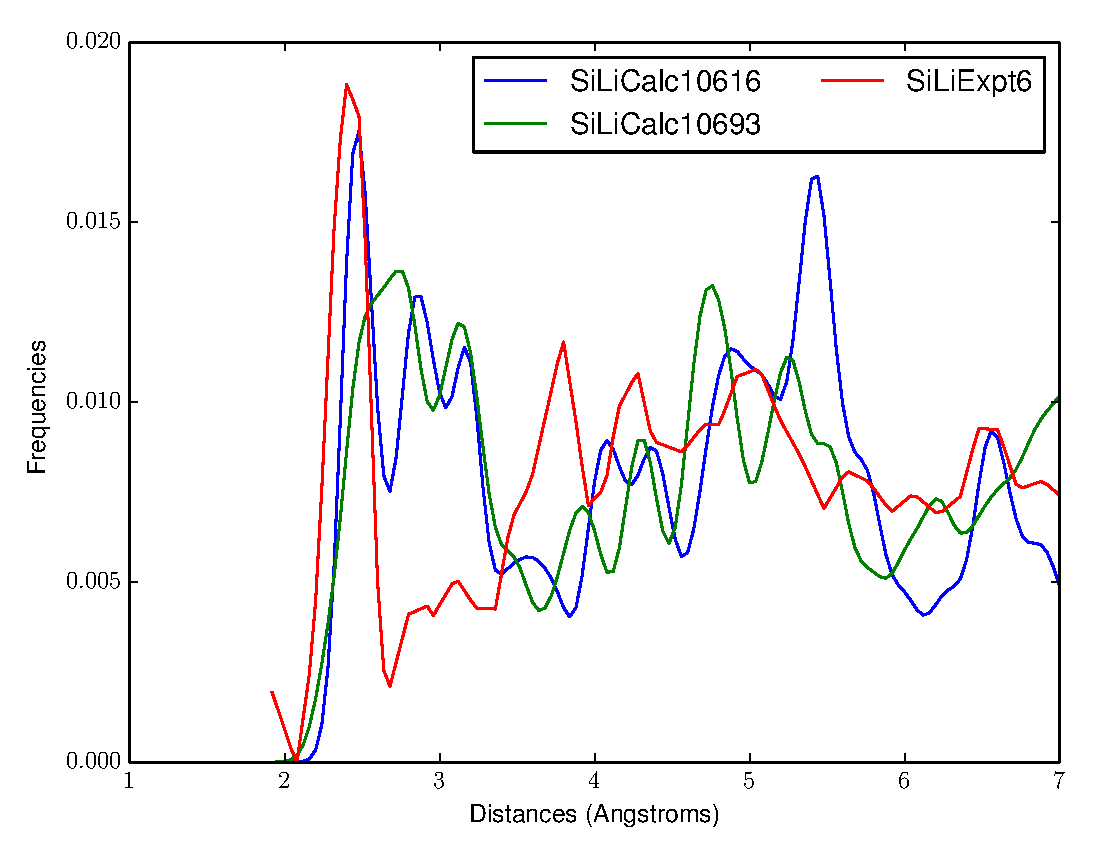
\includegraphics[scale=0.8]{figs/PC128MatchSiLiExpt6-SiLiCalc10616-SiLiCalc10693.eps}
\caption{PCA Matches: SiLiExpt6, SiLiCalc10616, SiLiCalc10693}
\end{center}
\end{figure}

\begin{figure}[ht]
\begin{center}
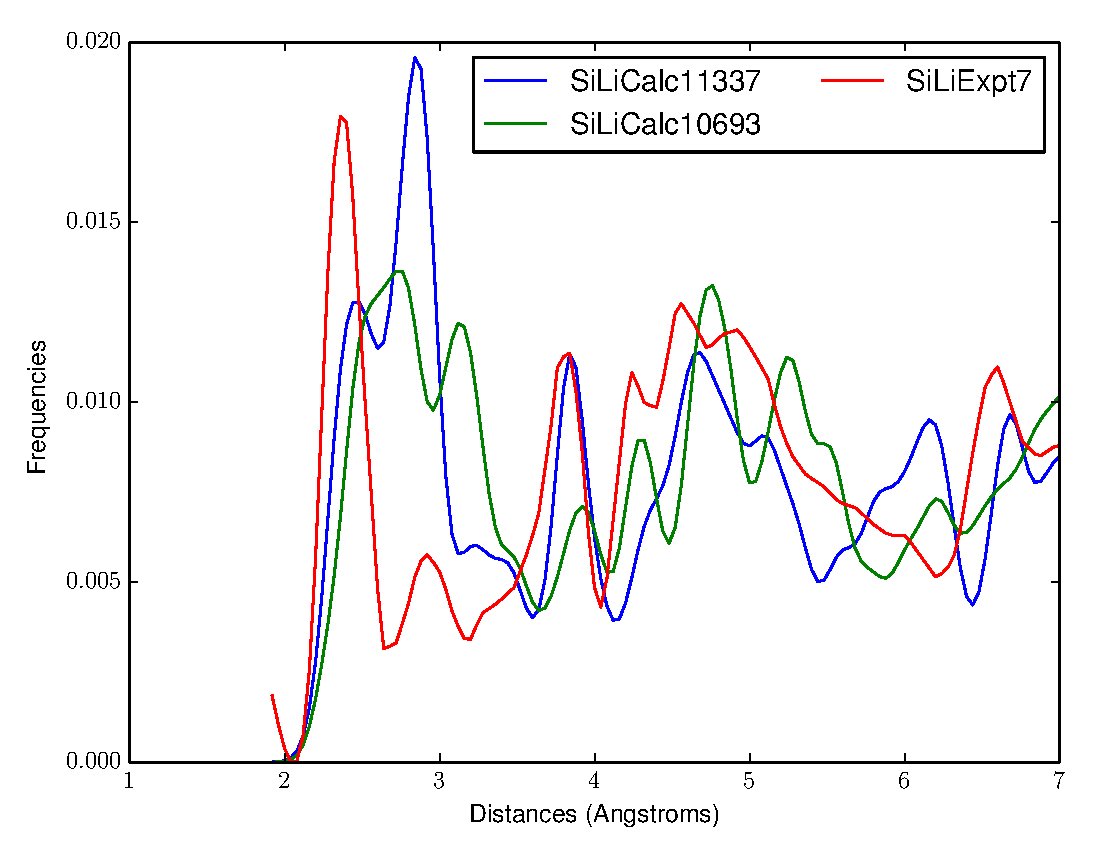
\includegraphics[scale=0.8]{figs/PC128MatchSiLiExpt7-SiLiCalc10693-SiLiCalc11337.eps}
\caption{PCA Matches: SiLiExpt7, SiLiCalc10693, SiLiCalc11337}
\end{center}
\end{figure}

\begin{figure}[ht]
\begin{center}
\includegraphics[scale=0.8]{figs/PC128MatchSiLiExpt8-SiLiCalc10693-SiLiCalc10651.eps}
\caption{PCA Matches: SiLiExpt8, SiLiCalc10693, SiLiCalc10651}
\end{center}
\end{figure}

\clearpage

\subsection{Synthetic Experimental Image Recognition}
\begin{figure}[ht]
  \begin{center}
    \includegraphics[scale=0.8]{figs/accuracy_with_pca.png}
    \caption{Synthetic Experimental Images Accuracy}
  \end{center}
\end{figure}

\begin{figure}[ht]
  \begin{center}
    \includegraphics[scale=0.8]{figs/accuracy_by_num_pc.png}
    \caption{Accuracy vs Number of Principal Components}
  \end{center}
\end{figure}
\clearpage

\section{Recognition Using Sparse Representations}
\subsection{Experimental Image Recognition}
\begin{table}[h]
  \begin{tabular}{|l|l|}
    \hline
    \textbf{Experiment} & \textbf{Match} \\ \hline
    ExptGaAs            & CalcGaAs       \\ \hline
    ExptInAs            & CalcInAs       \\ \hline
    SiLiExpt1           & SiLiCalc10001  \\ \hline
    SiLiExpt2           & SiLiCalc10001  \\ \hline
    SiLiExpt3           & SiLiCalc10001  \\ \hline
    SiLiExpt4           & SiLiCalc10003  \\ \hline
    SiLiExpt5           & SiLiCalc10003  \\ \hline
    SiLiExpt6           & SiLiCalc10616  \\ \hline
    SiLiExpt7           & SiLiCalc10382  \\ \hline
    SiLiExpt8           & SiLiCalc10382  \\ \hline
  \end{tabular}
  \caption{Experimental Image Recognition}
\end{table}

\begin{figure}[ht]
  \begin{center}
    \includegraphics[scale=0.8]{figs/SparseRepExptGaAs-CalcGaAs.eps}
    \caption{ExptGaAs, CalcGaAs}
  \end{center}
\end{figure}

\begin{figure}[ht]
  \begin{center}
    \includegraphics[scale=0.8]{figs/SparseRepExptInAs-CalcInAs.eps}
    \caption{ExptInAs, CalcInAs}
  \end{center}
\end{figure}

\begin{figure}[ht]
  \begin{center}
    \includegraphics[scale=0.8]{figs/SparseRepSiLiExpt1-SiLiCalc10001.eps}
    \caption{SiLiExpt1, SiLiCalc10001}
  \end{center}
\end{figure}

\begin{figure}[ht]
  \begin{center}
    \includegraphics[scale=0.8]{figs/SparseRepSiLiExpt2-SiLiCalc10001.eps}
    \caption{SiLiExpt2, SiLiCalc10001}
  \end{center}
\end{figure}

\begin{figure}[ht]
  \begin{center}
    \includegraphics[scale=0.8]{figs/SparseRepSiLiExpt3-SiLiCalc10001.eps}
    \caption{SiLiExpt3, SiLiCalc10001}
  \end{center}
\end{figure}

\begin{figure}[ht]
  \begin{center}
    \includegraphics[scale=0.8]{figs/SparseRepSiLiExpt4-SiLiCalc10003.eps}
    \caption{SiLiExpt4, SiLiCalc10003}
  \end{center}
\end{figure}

\begin{figure}[ht]
  \begin{center}
    \includegraphics[scale=0.8]{figs/SparseRepSiLiExpt5-SiLiCalc10003.eps}
    \caption{SiLiExpt5, SiLiCalc10003}
  \end{center}
\end{figure}

\begin{figure}[ht]
  \begin{center}
    \includegraphics[scale=0.8]{figs/SparseRepSiLiExpt6-SiLiCalc10616.eps}
    \caption{SiLiExpt6, SiLiCalc10616}
  \end{center}
\end{figure}

\begin{figure}[ht]
  \begin{center}
    \includegraphics[scale=0.8]{figs/SparseRepSiLiExpt7-SiLiCalc10382.eps}
    \caption{SiLiExpt7, SiLiCalc10382}
  \end{center}
\end{figure}

\begin{figure}[ht]
  \begin{center}
    \includegraphics[scale=0.8]{figs/SparseRepSiLiExpt8-SiLiCalc10382.eps}
    \caption{SiLiExpt8, SiLiCalc10382}
  \end{center}
\end{figure}
\clearpage

\subsection{Synthetic Experimental Image Recognition}
\begin{figure}[ht]
  \begin{center}
    \includegraphics[scale=0.8]{figs/SparseRepSynthExprAccuracy.png}
    \caption{Synthetic Experimental Image Recognition Accuracy}
  \end{center}
\end{figure}
\clearpage


\section{Sources}
\begin{verbatim}
http://en.wikipedia.org/wiki/Atom_vibrations
http://en.wikipedia.org/wiki/Radial_distribution_function
http://en.wikipedia.org/wiki/Weierstrass_transform
http://matplotlib.org/api/mlab_api.html
http://en.wikipedia.org/wiki/Principal_components_analysis
\end{verbatim}

%\pagebreak
%\noindent \textbf{Appendix}\\
%\emph{Convolution Commutativity}\\
%\begin{align*}
%&\int_{- \infty}^\infty f(\tau) g(t - \tau) d\tau\\
%&u = t - \tau\\
%&\tau = -\infty \rightarrow u = \infty\\
%&\tau = \infty \rightarrow u = -\infty\\
%&du = -d\tau\\
%&- \int_\infty^{-\infty} f(t - u) g(u) du = \int_{-\infty}^\infty g(u) f(t-u)du\\
%\end{align*}

\end{document}
